%!TEX root = ../../dissertation.tex
%%%%%%%%%%%%%%%%%%%%%%%%%%%%%%%%%%%%%%%%%%%%%%%%%%%%%%%%%%%%%%%%%%%%%%%%%%%%%%%%
\chapter{Evaluating Mobile Signaling Traffic and Load}
\label{chap:mobilenetsmeasuring}

With the architectural and methodological overview concluded this chapter can now move on to the actual evaluation. To this end, the previously described dataset is explored for any control plane load related signs. The evaluation, including a statistical analysis, is given in Section~\ref{c4:sec:evaluations}. The measurement data backs up a number of assumptions on the behavior of different device and operating system types, but also reveals some remarkable differences in signaling characteristics.

The results of these measurements are then used to construct a queuing theoretic load model for a \gls{CN} in Section~\ref{c4:sec:modeling}. This model is then extended with  virtualization modifications to it and followed by a numerical simulation in Section~\ref{c4:sec:simulation} to confirm the viability of the models.



%%%%%%%%%%%%%%%%%%%%%%%%%%%%%%%%%%%%%%%%%%%%%%%%%%%%%%%%%%%%%%%%%%%%%%%%%%%%%%%
%!TEX root = ../../dissertation.tex
%%%%%%%%%%%%%%%%%%%%%%%%%%%%%%%%%%%%%%%%%%%%%%%%%%%%%%%%%%%%%%%%%%%%%%%%%%%%%%%%
\section{Signaling Evaluation}
\label{c4:evaluations}

Finally, the core network control plane load evaluations are at hand. We evaluate the previously described dataset and iterate over several approaches to measure load and related factors.



%%%%%%%%%%%%%%%%%%%%%%%%%%%%%%%%%%%%%%%%%%%%%%%%%%%%%%%%%%%%%%%%%%%%%%%%%%%%%%%%
\subsection{Traffic Ratio Estimations}


\begin{table}
\centering
\caption{Relative traffic statistics extracted from the dataset.}
\label{tab:trafficstats}
    \begin{tabu}{XX[r]X[r]X[r]X[r]X[r]}
    \toprule
    & \textbf{Flows} & \textbf{Traffic} & \textbf{Tunnels} & \textbf{\gls{gtp} pairs} & \textbf{Devices}\\ 
    \midrule
    \multicolumn{2}{c}{\textbf{By device type}}       &             &             &             &           \\
%    In TAC DB      & $99.72\%$   & $99.97\%$   & $87.57\%$   & $90.95\%$   & $80.93\%$ \\
    Smartphones      & $20.58\%$   & $12.81\%$   & $60.31\%$   & $75.99\%$   & $37.97\%$ \\
    Regular phones   & $0.26\%$    & $0.37\%$    & $5.40\%$    & $0.94\%$    & $9.25\%$  \\
    \gls{3G} dongles & $66.55\%$   & $75.12\%$   & $12.71\%$   & $9.53\%$    & $25.10\%$ \\
    \midrule
    \textbf{By \gls{os}}&          &             &             &             &           \\
    Android          & $10.82\%$   & $6.48\%$    & $14.33\%$   & $43.33\%$   & $14.01\%$ \\
    iOS              & $7.22\%$    & $4.47\%$    & $18.91\%$   & $20.35\%$   & $7.94\%$  \\
    Symbian          & $1.02\%$    & $1.09\%$    & $21.17\%$   & $4.51\%$    & $12.97\%$ \\
    Blackberry OS    & $0.07\%$    & $0.10\%$    & $2.17\%$    & $2.60\%$    & $1.48\%$  \\
    \bottomrule
    \end{tabu}
\end{table}

To get a first grasp of the dynamics present in the dataset and the core network under investigation, Figure~\ref{tab:trafficstats} shows a small survey of the traffic composition split up by device type and \gls{os} categories. The majority of signaling messages originated from smartphones, which in turn generated only a small portion of user traffic when compared to \gls{3G} dongles.

With these numbers, the notion of active devices or tunnels can also be introduced. This only includes entities that, besides signaling, actively generated user traffic during their life cycle. Interestingly, only about $82\%$ of all unique devices in the trace were active and could be associated with at least one traffic flow. The remaining $12\%$ of devices still had an open \gls{gtp} tunnel but never used it. This is an extreme for the core network, as it causes a significant amount of control plane load without any actual benefit to either the network or the device. The active device distinction will als be used later on in the evaluation.

Unfortunately, the dataset does not contain any hard numbers on the volume of the signaling messages, which could be a direct indicator of the network load the control plane imposes. But using the estimation of the upper limit of a \gls{gtp} message from Section~\ref{c4:sec:gtp}, a rough upper limit on the total signaling traffic can also be derived. The following formula is used:

\begin{align}
\phantom{,}v_s &=& 2\left|S\right|(v_{gtp} + v_{udp} + v_{ip})\text{,}\\
\phantom{.}t_r &=& \frac{v_s}{v_t} \approx 0.7\%\text{,}
\end{align}

with the signaling volume $v_s$, the set of signaling messages $S$, the estimated size of a \gls{gtp} message $v_s$, and the length of the \gls{UDP} and \gls{IP}headers. In this scenario, the traffic ratio $t_r$ of $v_s$ compared to the total traffic $v_t$ is calculated to be a minute $0.7\%$. Therefore, it can be safely assumed that the volume of control plane traffic appears to be a non-issue and not the bottleneck.The other load factors at the network nodes described earlier must play a more critical role, such as the memory profile of the states kept in the gateway nodes, the time required to process the large number of information held in the messages, or the imposed latency through several message round trips during transactions.

This is why the following evaluations are all intended to find some indirect approach to measure the system's load.



%%%%%%%%%%%%%%%%%%%%%%%%%%%%%%%%%%%%%%%%%%%%%%%%%%%%%%%%%%%%%%%%%%%%%%%%%%%%%%%%
\subsubsection{\texorpdfstring{\acrshort{gtp}}{GTP} Tunnel Duration}

The first indirect evaluation target will be the duration of the \gls{gtp} tunnels. This duration is directly related to the amount of occurring tunnel management signaling between the \gls{SGSN} and \gls{GGSN}. In turn, each of these signaling interactions causes processing at the two involved nodes and changes the amount of state in the form of the \gls{PDP} context. In terms of signaling messages, looking at the duration catches both tunnel create and delete messages, but no update message.

For the purpose of the evaluation the duration is defined as the interval between corresponding \gls{gtp} create and delete messages. As soon as the \gls{GGSN} sends its successful response to the create request, it can be expected that the necessary state has been created throughout the \gls{CN} and is ready to forward user packets. Similarly, after a delete message, user traffic should not be forwarded anymore. However, state may still exist and could be freed up lazily. But the latter depends entirely on the specific implementation.

As a side note, while the trace itself is only one week long, information on tunnels longer than this period can still be obtain when they were closed during the period. The trace's record on delete messages also contains the timestamp of the initial tunnel creation.


All the individual tunnel durations in the dataset are differentiated based on two factors based on the presented \gls{TAC} mechanics. The first part of the investigation looks at tunnels from different device types. After that,possible influences from the operating system are investigated. Both categorizations should prove valuable for example in deciding if currently some phone types put more signaling load on the network and to direct measures to improve this situation.



%%
\paragraph{Influence of the Device Type}

% ! <-- !

\begin{figure}[htb]
    \centering
    \includegraphics[width=\textwidth]{images/R-tunnel-duration-device-type.pdf}
    \caption{Tunnel duration distribution, separated for 3G dongles, smartphones and regular phones with medians at \SI{115}{\second} (Total), \SI{31}{\second} (Regular), \SI{82}{\second} (Smartphone), and \SI{1207}{\second} (\gls{3G} Dongle)}
    \label{c4:fig:cdf-duration-device-class}
\end{figure}

Figure~\ref{c4:fig:cdf-duration-device-class} shows the empirical cumulative distribution functions for the \gls{PDP} Context durations in our dataset. We distinguish the total duration distribution as well as the the distributions for smartphones, regular phones, and \gls{3G} dongles. It can be observed that tunnel durations range between  seconds and more than one week.

The median differs between device types, being much longer for \gls{3G} dongles than for mobile phones. This can probably be expected, as typical dongle sessions might involve working at a laptop for periods longer than a few seconds or minutes. Also for the dongles, we observe less extremely long tunnels with durations above several hours. Again, we could hypothetically relate this to a usual laptop working environment, where the device is used for a few hours but then shut down. With this, the \gls{PDP} Context is deleted as well. Interestingly, the median duration of regular phones is higher than that of smartphones. This may indicate that  smartphones regularly (and perhaps automatically) cause data traffic and therefore tunnels to occur. We conjecture this to be a first indication of the ``Angry Birds'' effect of automatically transferring small amounts of data, e.g. weather reports, stock exchange data, \gls{RSS} feeds, or email notifications. We also observe two distinct steps, one at \SI{6.8}{\second} for dongles, and one at \SI{30}{\minute} in the overall and smartphone distributions. While we do not have a plausible explanation for the former, the latter could be explained by a value chosen for the \gls{RRC} state machine transition to the IDLE state (cf. Figure \ref{c4:fig:rrcstatemodel}).

%%

Figure~\ref{c4:fig:cdf-duration-device-class} shows the empirical cumulative distribution functions for the \gls{PDP} Context durations in our dataset. We distinguish the total duration distribution as well as the the distributions for smartphones, regular phones, and \gls{3G} dongles. It can be observed that tunnel durations range between mere seconds and more than one week\footnote{Although our dataset is just one week long, some tunnels started before the beginning of that week, and ended within it. Since the tunnel start dates were still available from the system, we chose to include the data.}.

The median is clearly different between device types, being much longer for \gls{3G} dongles than for mobile phones. This can probably be expected, as typical dongle sessions might involve working at a laptop for periods longer than a few seconds or minutes. Also, for the dongles, we observe less extremely long tunnels. Again, we could relate this to a hypothetical laptop working environment, where the device is used for a few hours but then shut down. With this, the \gls{PDP} Context is deleted as well. 

Interestingly, the median duration of regular phones is higher than that of smartphones. This may indicate that smartphones regularly (and perhaps automatically) cause data traffic and therefore tunnels to occur. We conjecture this to be a first indication of the ``Angry Birds'' effect of automatically transferring small amounts of data, e.g. weather reports, stock exchange data, \gls{RSS} feeds, or email notifications. We also observe two distinct steps, one at \SI{6.8}{\second} for dongles, and one at \SI{30}{\minute} in the overall and smartphone distributions.



%%
\paragraph{Influence of the \texorpdfstring{\acrshort{os}}{OS}}

\begin{figure}[htb]
    \centering
    \includegraphics[width=1.0\textwidth]{images/R-tunnel-duration-operating-system.pdf}
    \caption{Tunnel duration cumulative distribution function, separated for Android and iOS devices; Medians at \SI{115}{\second} (Total), \SI{15.5}{\second} (Symbian), \SI{104}{\second} (iOS), and \SI{765}{\second} (Android)}
    \label{c4:fig:cdf-duration-os}
\end{figure}

%iOS: over 20\% of tunnels shorter than two seconds. 

Taking an even closer look at the smartphone device fraction, we can still observe major differences as depicted in the empirical cumulative distribution functions of Figure~\ref{c4:fig:cdf-duration-os}. The tunnel duration distribution of the Symbian device fraction behaves much closer to the regular phones already depicted in Fig.~\ref{c4:fig:cdf-duration-device-class}. A possible explanation could be the user-base being more traditional, or the devices being feature phones whose behavior clearly differs from smartphones.

Again, a number of steps are visible in the distributions. %Steps at multiples of 10 seconds indicate that timer-induced transitions happen. 
Those steps that are only visible in one operating system type point to a source involving the phone rather the network. This especially includes the \SI{30}{\second}, \SI{300}{\second}, and \SI{600}{\second} steps (i.e. accumulations of incidents) for Android, and the \SI{600}{\second} step for iOS devices. However, whether this behavior should be attributed to the operating systems themselves cannot be decided by only looking at these distribution. Other factors, e.g. the device's firmware version and user traffic dynamics need also be observed. We leave this point for future work.

A last artifact of note are the larger number of iOS devices with very short tunnel durations. Over $20\%$ of all tunnels established by these devices are shorter than two seconds. While the actual cause still remains unknown, it could be an interaction between short regular traffic burst and \gls{3GPP} Fast Dormancy \cite{gsma2011fdbestpract} which iOS devices are known to implement. Fast Dormancy is a technique to release radio resources more quickly. It is deemed to improve device battery life, radio signaling and radio spectrum efficiency. However, due to the earlier and more frequent transition to the IDLE state, it also could cause an increase in core network tunnel management signaling, which is probably what happened in the iOS case depicted in the \gls{ECDF}.

%%

Taking an even closer look at the smartphone device fraction, and differentiating the operating system to Symbian, Android, and iOS, we can still observe major differences as depicted in the empirical cumulative distribution functions of Figure~\ref{c4:fig:cdf-duration-os}. The tunnel duration distribution of the Symbian device fraction behaves much closer to the regular phones already depicted in Fig.~\ref{c4:fig:cdf-duration-device-class}. A possible explanation could be the user-base being more traditional, or the devices being feature phones whose behavior clearly differs from smartphones.

Again, a number of steps (i.e. accumulations of incidents) are visible in the distributions. Those that are only visible in one operating system type point to a source involving the device rather the network. This especially includes the \SI{30}{\second}, \SI{300}{\second}, and\SI{600}{\second} steps for Android, and the \SI{600}{\second} step for iOS devices. However, whether this behavior should be attributed to the operating systems themselves cannot be decided by only looking at these distribution. Other sources, e.g. the device's firmware version and user traffic dynamics need also be observed.

A last artifact of note are the large number of iOS devices with very short tunnel durations. Over $20\%$ of all tunnels established by these devices are shorter than two seconds. Our working hypothesis is, that this is an interaction between short regular traffic burst and a form of Fast Dormancy \cite{gsma2011fdbestpract} which iOS devices are known to implement, a technique to explicitly release radio resources. It is deemed to improve device battery life, radio signaling and radio spectrum efficiency. However, due to the earlier and more frequent radio state changes, it also could cause an increase in core network tunnel management signaling, which is probably what happened in the iOS case depicted in the \gls{CDF}.




%%
\paragraph{Influence of \acrshort{RAT} and other factors}
Explain, why it is not here.
%%
%TODO: radio access type plots, if we have the data
%
%\begin{figure}
%\centering
%\includegraphics[width=\columnwidth]{figures/tunnel-dur-radio-cdf-mod.pdf}
%\caption{Tunnel duration distribution, separated for UMTS and GPRS radio access [NOTE: only in the last tunnel segment; and majority of radio types %is unknown anyway.}
%\label{fig:cdf-duration-radio}
%\end{figure}

% 10/30m jumps can be seen on android, but not on iOS, why?
%  maybe fast dormancy?



%%
\paragraph{Influence Strength of the Categories}


\begin{figure}[htb]
        \centering
        % \begin{subfigure}[b]{0.50\textwidth}
        %         \centering
        %         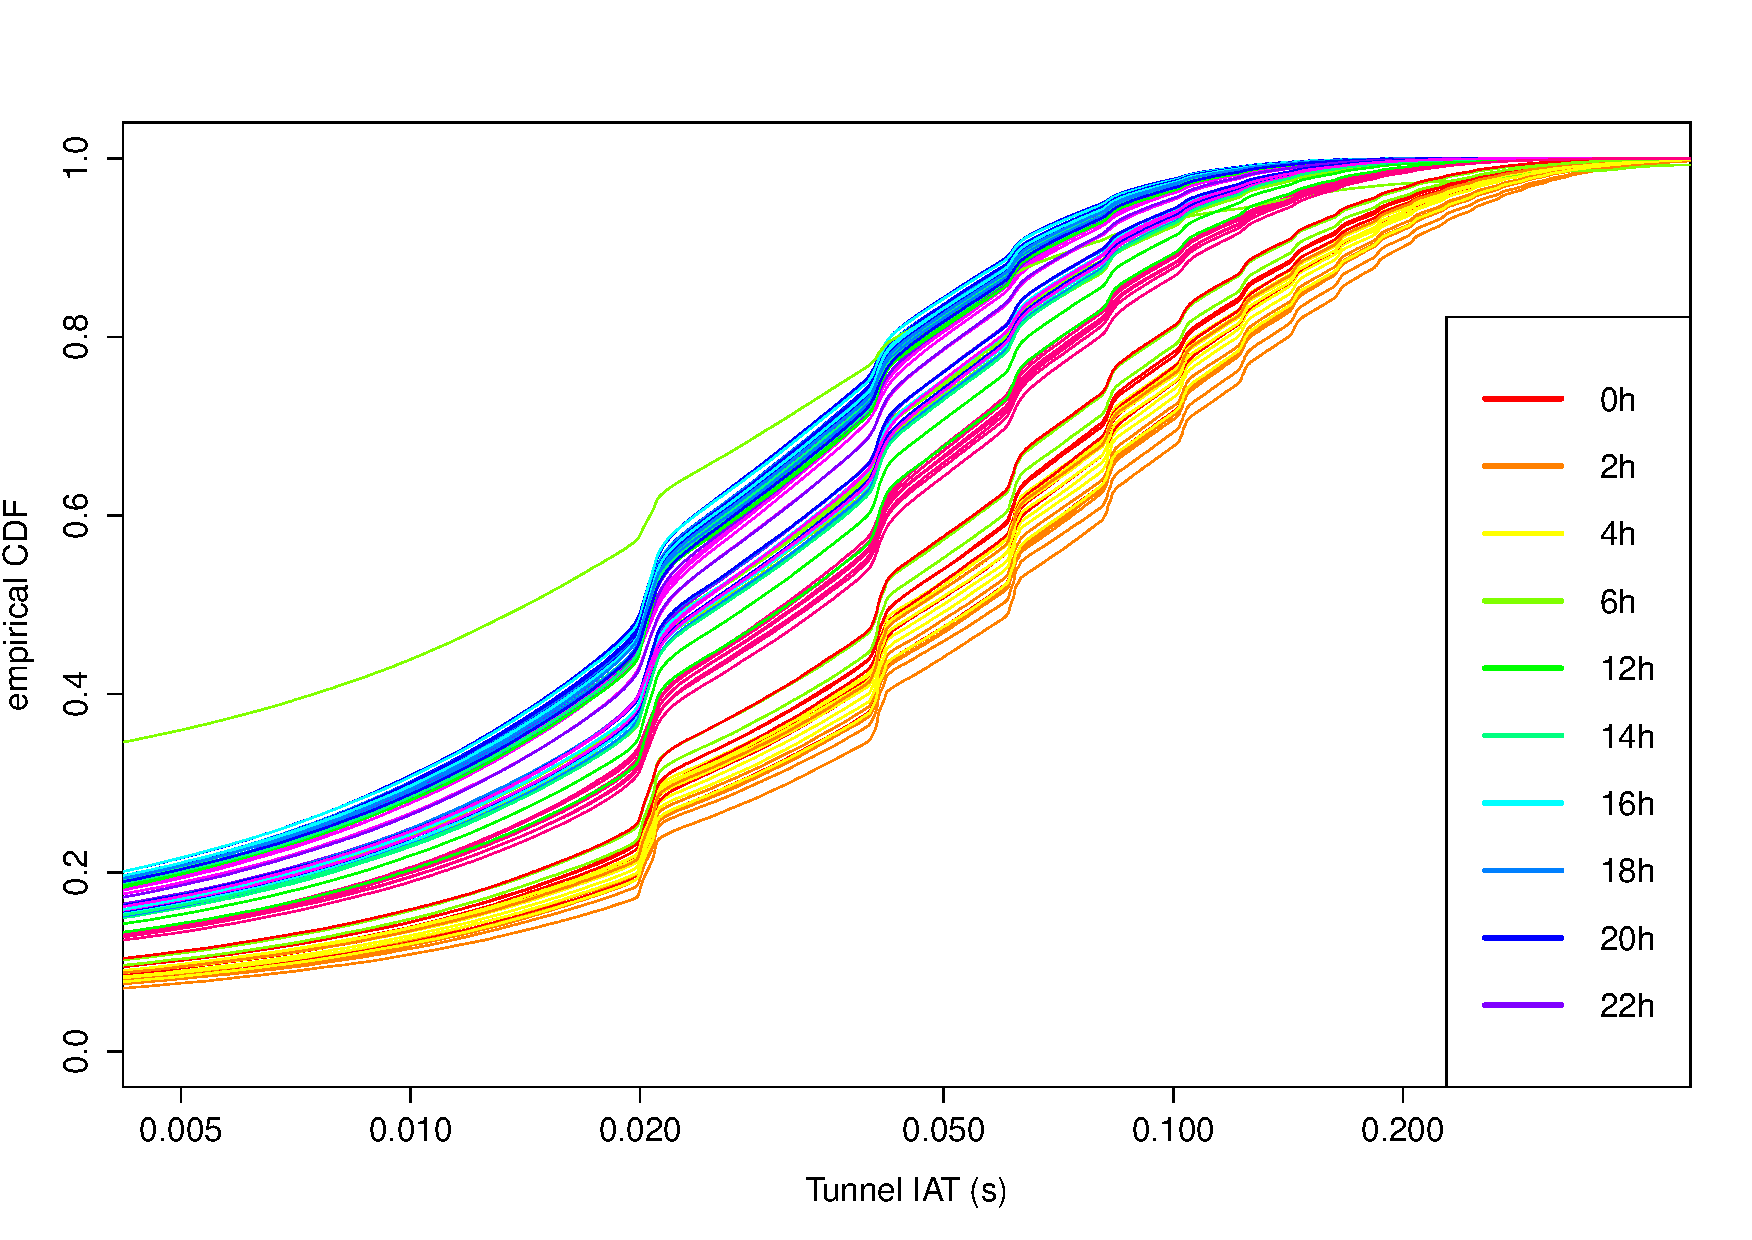
\includegraphics[width=\textwidth]{figures/R-IAT-ecdf-2h-log.png}
        %         \caption{All incoming tunnel requests.}
        %         \label{fig:IAT-ecdf-2h-all}
        % \end{subfigure}%
        %~ %add desired spacing between images, e. g. ~, \quad, \qquad etc.
          %(or a blank line to force the subfigure onto a new line)
        \begin{subfigure}[b]{0.50\textwidth}
            \centering
            \includegraphics[width=\textwidth]{images/qq-total-vs-android.pdf}
            \caption{Android duration over the total duration.}
            \label{c4:fig:qq-total-vs-android}
        \end{subfigure}%
        ~
        \begin{subfigure}[b]{0.50\textwidth}
            \centering
            \includegraphics[width=\textwidth]{images/qq-total-vs-ios.pdf}
            \caption{iOS duration over the total duration.}
            \label{c4:fig:qq-total-vs-ios}
        \end{subfigure}

        \begin{subfigure}[b]{0.50\textwidth}
            \centering
            \includegraphics[width=\textwidth]{images/qq-total-vs-dongle.pdf}
            \caption{3G Dongle duratio over the total duration.}
            \label{c4:fig:qq-total-vs-dongle}
        \end{subfigure}%
        ~
        \begin{subfigure}[b]{0.50\textwidth}
            \centering
            \includegraphics[width=\textwidth]{images/qq-total-vs-smartphone.pdf}
            \caption{Smartphone duration over the total duration.}
            \label{c4:fig:qq-total-vs-smartphones}
        \end{subfigure}
 \caption{Q-Q Plots of the tunnel duration distributions per operating system, with encircled deciles.}
\label{c4:fig:qq-plots}
\end{figure}

In an attempt to show which of the presented categories have an impact on the total duration (if at all), we present Q-Q plots of the various categorized durations against the total duration in Figure~\ref{c4:fig:qq-plots}. In theory, if both durations follow the same distribution, one expects a straight line through the origin at an angle of 45$^o$. A steeper incline indicates less densely spaced values in the distribution at the y axis. Looking at igures~\ref{c4:fig:qq-total-vs-android} and \ref{c4:fig:qq-total-vs-ios} which compare different operating systems, both similar and dispersing parts can be observed. While tunnel durations on Android  are more similarly distributed for the shorter and longer durations, iOS device tunnel durations are most similar to the overall tunnel duration distribution in the middle range of values.

Combining all types of smartphones together and comparing them to the other major player in any mobile network, the 3G dongles, we observe in Figure \ref{c4:fig:qq-total-vs-smartphones} that both the total and the smartphone durations are almost equally distributed (except for minor variations). On the other hand, 3G dongles follow a very different distribution, see Figure \ref{c4:fig:qq-total-vs-dongle}. Their effect on tunnel management signaling seems to be negligible despite the  large amount of traffic they are causing. Therefore, we conclude that planning and dimensioning of the control plane needs to keep smartphone behaviors more closely in mind than that of other device types.


\begin{figure}[htb]
	\centering
	\includegraphics[width=1.0\textwidth]{images/stacked-durations-2-fixed.pdf}
	\caption{Stacked logscale bin plot of the number of tunnels with duration in this bin; classified by Android, iOS and 3G dongles.}
	\label{c4:fig:stacked-durations}
\end{figure}

Figure~\ref{c4:fig:stacked-durations} shows another interesting influence the operating system has on signaling in the mobile core network. This plot shows the relative number of tunnels with a duration in one of 1000 logarithmically scaled bins, stacked by OS category on top of each other. As with the separate distributions, we discover that the durations are not evenly distributed, but rather follow sharp spikes. The largest spike across all categories is the one at a duration of 30 minutes, making up about 1.8\% of all tunnels in the network. Since this spike happens across all device types, we think this makes a rather strong case for being network-induced, and an indication for the aforementioned possible IDLE state transition. On the other hand, the bulk in the short-to-medium ranges of tunnel duration is rather not governed by the two major smartphone operation systems but by other devices in the network, which do not show major spikes in other bins. We can also recognize a long-tail behavior in the distribution of tunnel durations.






%%%%%%%%%%%%%%%%%%%%%%%%%%%%%%%%%%%%%%%%%%%%%%%%%%%%%%%%%%%%%%%%%%%%%%%%%%%%%%%
\subsubsection{\texorpdfstring{\acrshort{gtp}}{GTP} Tunnel Arrivals}

NOTE: IAT cannot be realistically be conducted with categories and still relate to the total system load.

Having characterized the dataset available to us we now shed some light on the control plane and load dynamics in a mobile core network and attempt to show the possible impact of certain devices or other properties of the network. 



While tunnel durations and the involved signaling at the beginning and end of the duration is one aspect of control plane load, the number of tunnel arrivals might be another, which we are looking into in this section.

In addition to describing the arrival process on the basis of the number of arrivals, we also take a look at the tunnel inter-arrival time. Specifically, with this process we mean the arrival of tunnel requests, i.e. GTP CREATE requests, at the \gls{GGSN}. This also adds to the foundation of the load model constructed in the next chapter. 

\begin{figure}[htb]
	\centering
	\includegraphics[width=\columnwidth]{images/create_freq.pdf}
	\caption{Tunnel arrivals in one second intervals.}
	\label{c4:fig:freq-arrivals}
\end{figure}

Figure \ref{c4:fig:freq-arrivals} depicts the number of arrivals per second during the whole weeklong period. Of note is the clear bimodal nature with one peak around twelve and the other in the low thirties. While the distribution is rather compact around these two peaks, there are some clear outliers up to 107.
If we again hypothesize that an increased number of arrivals means higher load in the network, we can assume that load is not constant but rather switches between two modes with some periods with extraordinary load induced by an increased number of arrivals.

\begin{figure}[htb]
	\centering
	\includegraphics[width=\columnwidth]{images/R-createspersecond-1h-violin.pdf}
	\caption{Violin plot of tunnel arrivals in one second per time of day.}
	\label{c4:fig:freq-arrivals-per-second-violin}
\end{figure}

To find the cause of these two modes we take a peek at the diurnal arrival pattern. Figure \ref{c4:fig:freq-arrivals-per-second-violin} contains a violin plot showing again the arrivals per second but broken down by time of day. A violin plot, while being similar to a box plot, additionally shows the density of the individual items on the vertical axis.
The nocturnal median from around midnight to 5am and the longer daytime median, 8am to 19pm, closely resemble the two modes found in the histogram. In between are short transition phases. Notably, during daytime the arrivals and their densities are spread out on a much larger value range. This could be an indication of load fluctuations in the system.


\begin{figure}[htbp]
        \centering
\makebox[\textwidth]{        
        \begin{subfigure}[b]{0.45\paperwidth}    
                \centering
                \includegraphics[width=\textwidth]{images/R-IAT-all-2h-ecdfs.pdf}
                \caption{All tunnel requests.}
                \label{c4:fig:IAT-ecdf-2h-all}
        \end{subfigure}%
        ~
        \begin{subfigure}[b]{0.45\paperwidth}
                \centering
                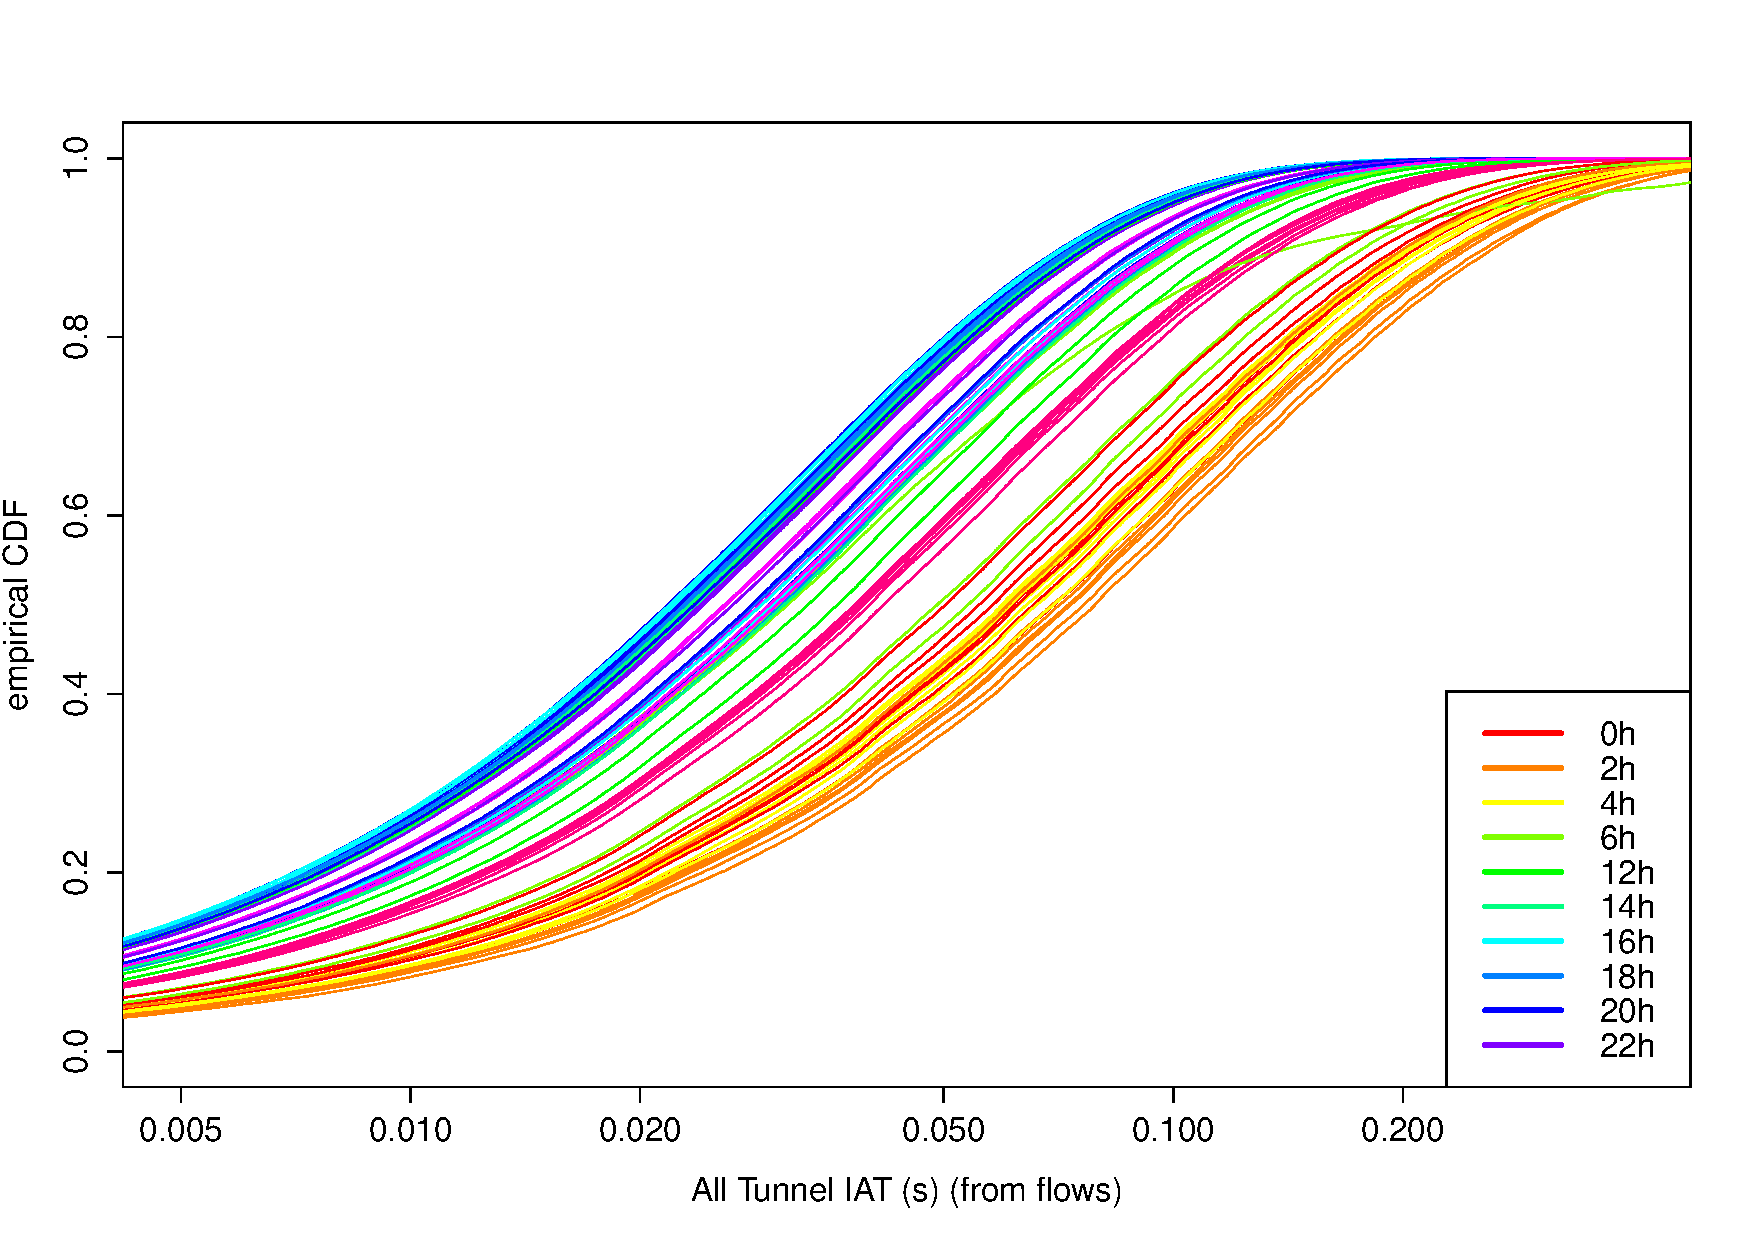
\includegraphics[width=\textwidth]{images/R-IAT-fromflows-ecdfs-2h.pdf}
                \caption{Only tunnels with data flows.}
                \label{c4:fig:IAT-ecdf-2h-active}
        \end{subfigure}
        }

 \makebox[\textwidth]{    
        \begin{subfigure}[b]{0.45\paperwidth}
                \centering
                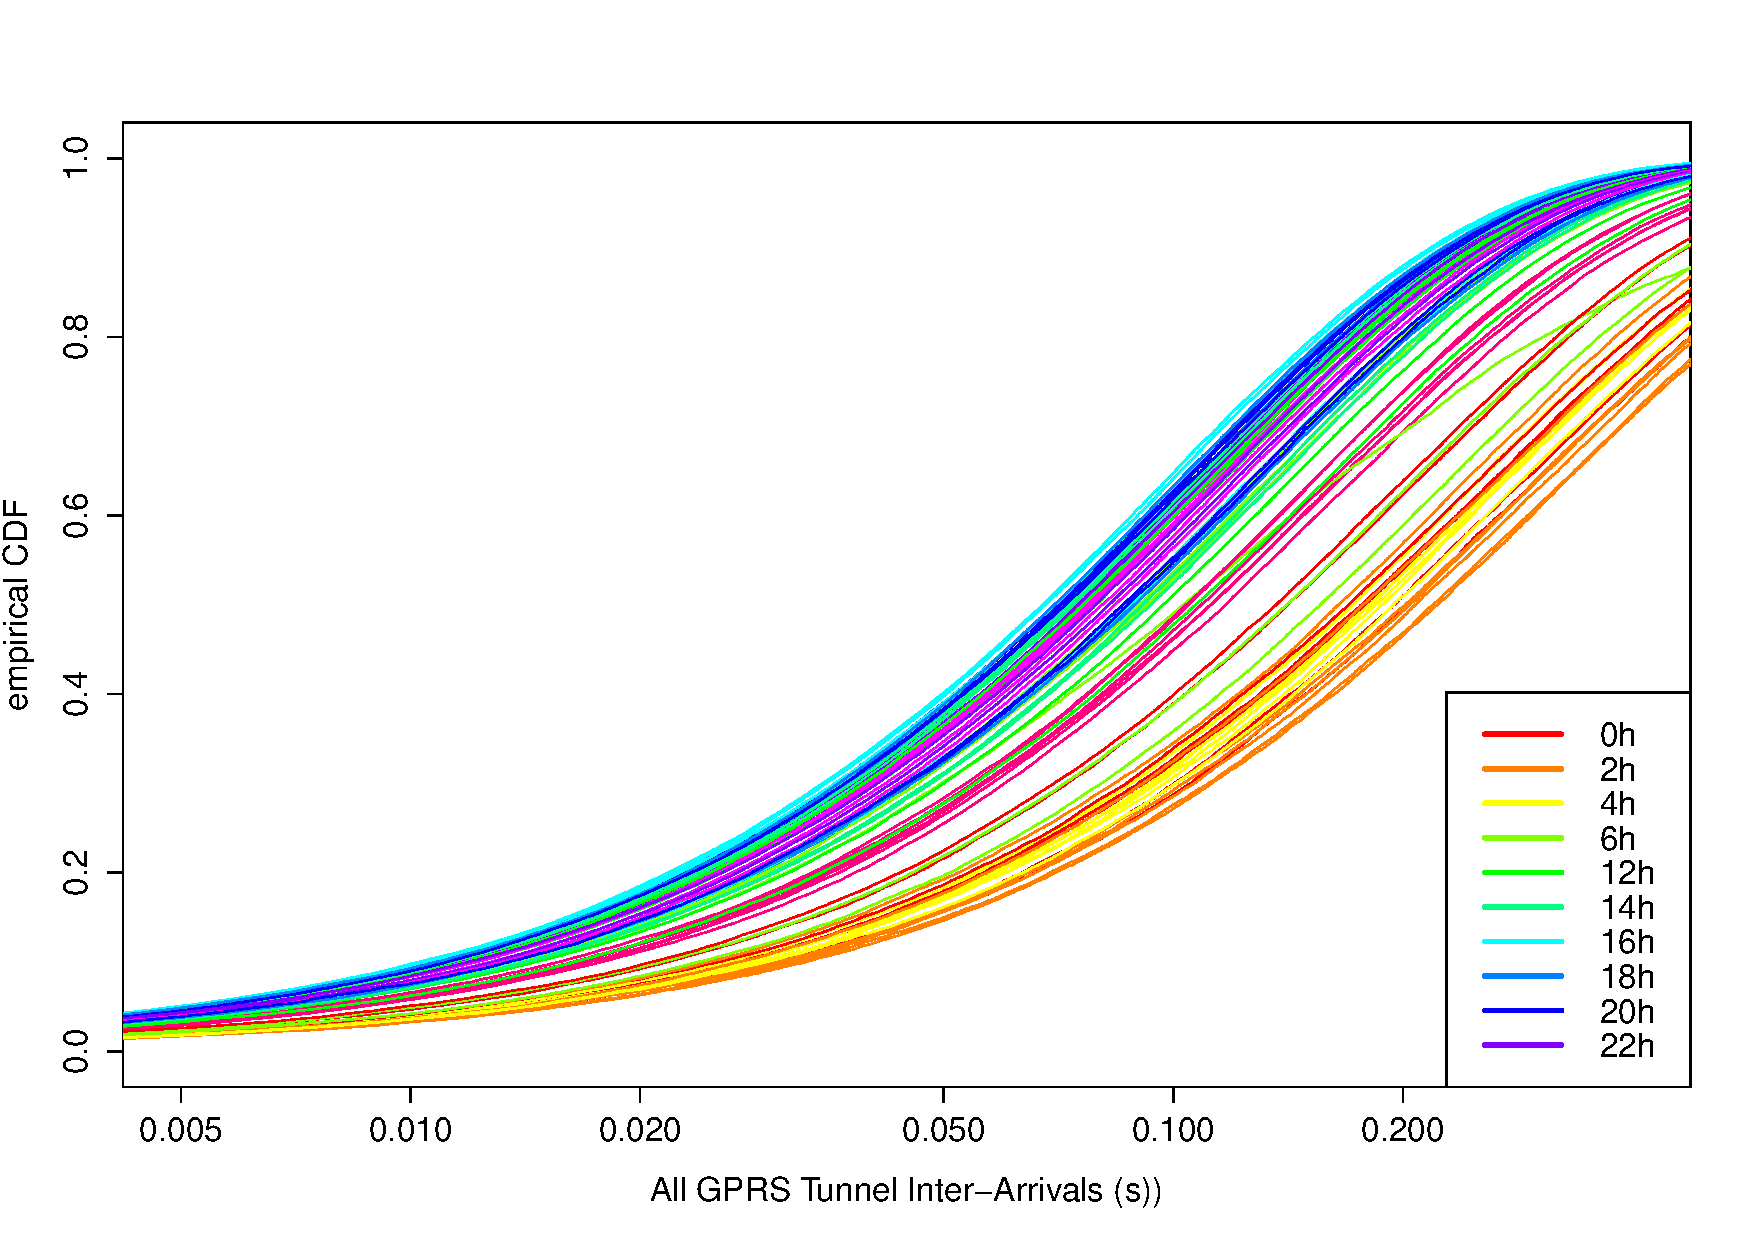
\includegraphics[width=\textwidth]{images/R-IAT-fromflows-gprs-ecdfs-2h.pdf}
                \caption{Tunnels with data flows initiated in GPRS.}
                \label{c4:fig:IAT-ecdf-2h-active-gprs}
        \end{subfigure}%
        ~
        \begin{subfigure}[b]{0.45\paperwidth}
                \centering
                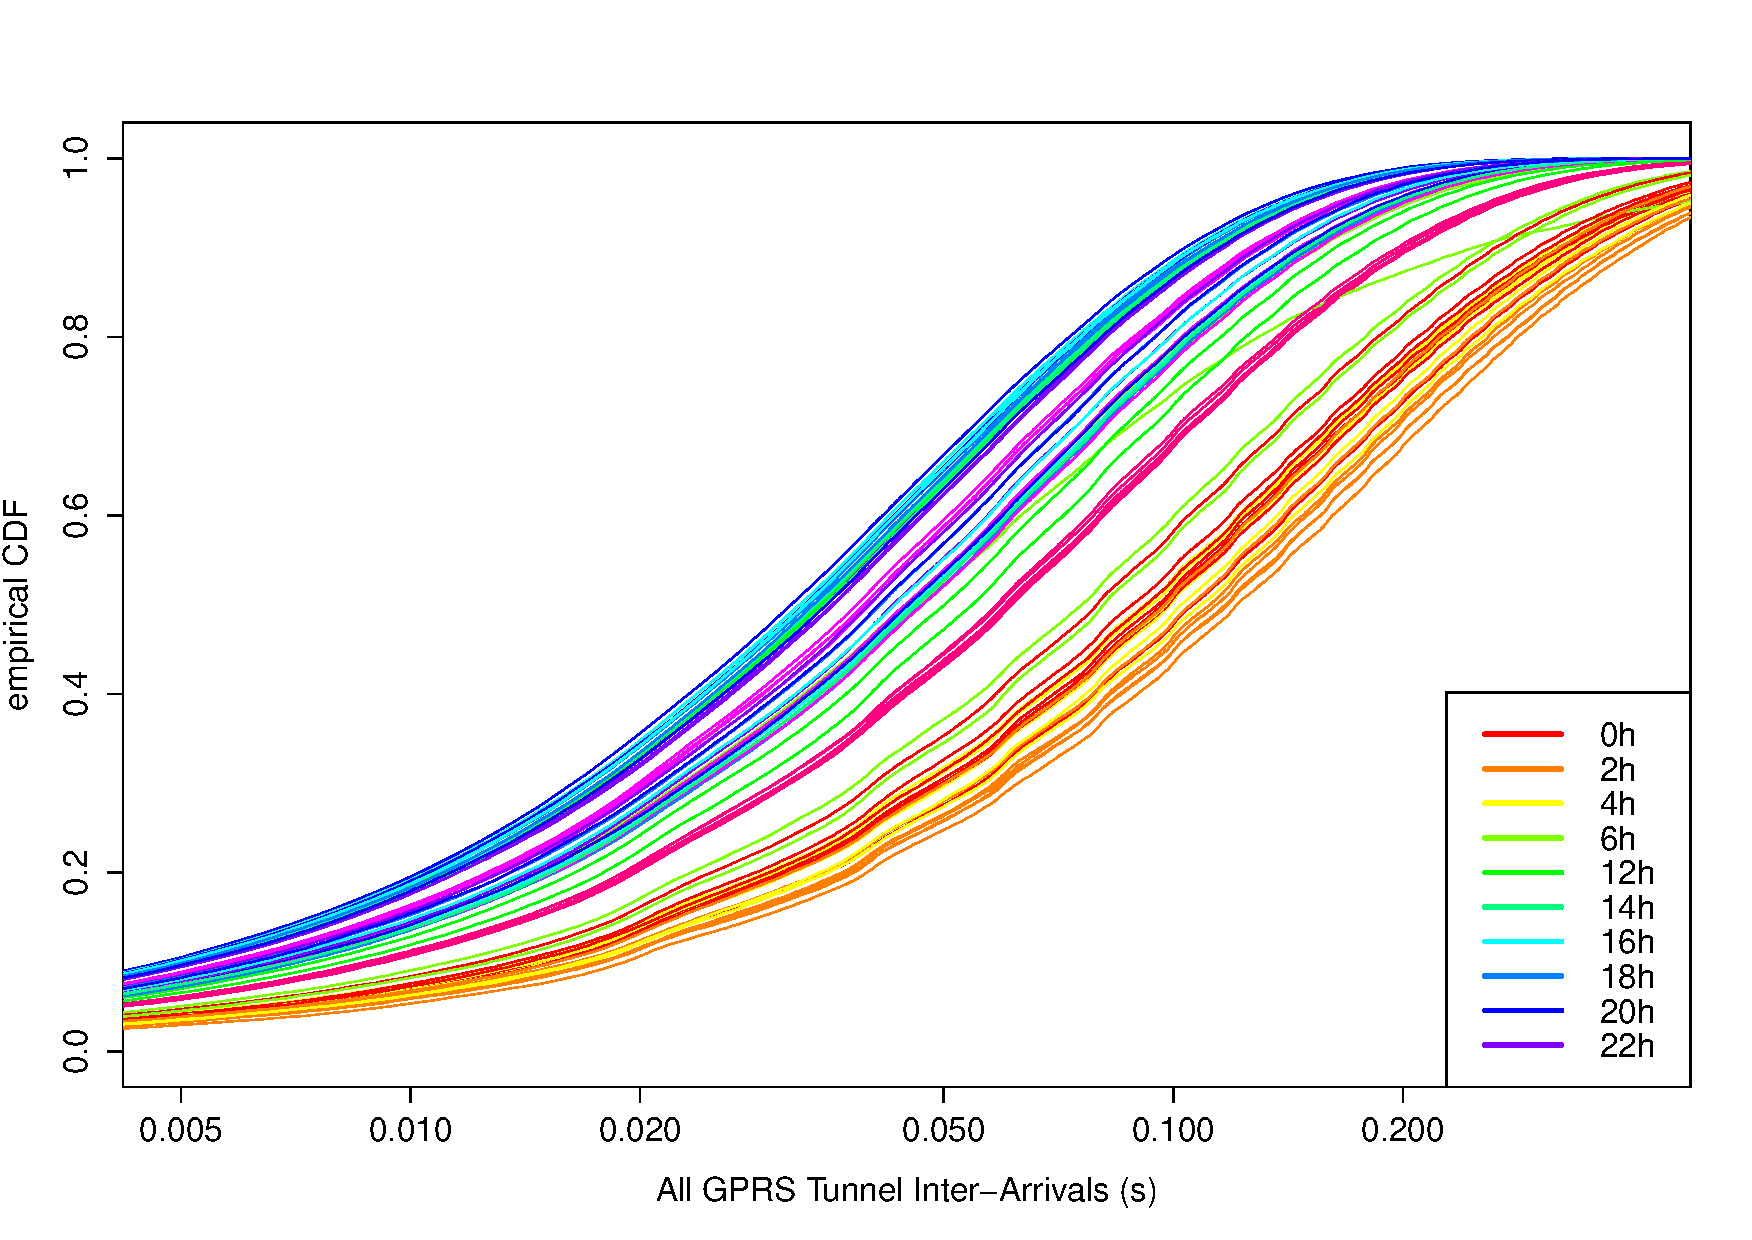
\includegraphics[width=\textwidth]{images/R-IAT-fromflows-umts-ecdfs-2h.pdf}
                \caption{Tunnels with data flows initiated in UMTS.}
                \label{c4:fig:IAT-ecdf-2h-active-umts}
        \end{subfigure}
}
        \caption{Empirical cumulative distribution function of the tunnel inter-arrival time in seconds by time of day for each day of one week.}
        \label{c4:fig:IAT-ecdf-2h}
\end{figure}

To investigate the arrivals from yet another angle we take a look at inter-arrival time of the tunnels in Figure~\ref{c4:fig:IAT-ecdf-2h}. This metric is more suited to describe the arrival process in the toy queuing model we propose. The empirical CDFs are again broken down by time of day, the same diurnal load oscillation can be observed. The medians range between about 20 and 60 milliseconds. Figure~\ref{c4:fig:IAT-ecdf-2h-all}, which represents all tunnel requests that the \gls{GGSN} received, shows wave-like steps in 20ms intervals in the plot. As this is happening very regularly at every time of the day we believe, that this effect must be from a source inside the mobile network and not induced from the outside, .e.g. through mobile devices.

This becomes even more peculiar when further breaking down the tunnel arrivals. We now distinguish between active tunnels, i.e. tunnels, that actually transported user traffic during their lifetime (cf. Fig.~\ref{c4:fig:IAT-ecdf-2h-active}), and active tunnels, which were created while having a GPRS (Fig.~\ref{c4:fig:IAT-ecdf-2h-active-gprs}) or UMTS (Fig.~\ref{c4:fig:IAT-ecdf-2h-active-umts}) connectivity, respectively. Note that only about 86\% of requested and created tunnels where actually used for user data transmissions afterwards. The 20ms-steps occur strongest when observing all tunnel arrivals, in a weaker form it is also present in the active and \gls{UMTS} tunnel portion. 

Our working hypothesis as to the origin of the effect is the \gls{TTI}. This time indicates the duration of a radio transmission and is usually either 10 or 20 milliseconds in length. It is also in sync for the whole network of base stations making the \gls{TTI} noticeable even when not measuring directly at the radio link. The observed step-width of 20ms therefore indicates, that the signaling procedure the GTP CREATE is part of, includes at least one trip from the mobile device over the radio interface. This makes sense, as the tunnel is typically created during the GPRS Attach procedure, which is indeed initiated at the user's device. Unfortunately, this also makes the tunnel arrivals come in somewhat batched, which could momentarily increase the load at the \gls{GGSN} that then would need to process more requests at once than if the arrivals followed a smooth stochastic distribution.




%%%%%%%%%%%%%%%%%%%%%%%%%%%%%%%%%%%%%%%%%%%%%%%%%%%%%%%%%%%%%%%%%%%%%%%%%%%%%%%
\subsection{\texorpdfstring{\acrshort{gtp}}{GTP} Tunnel Event Processing Time}

This brings us to another and potentially more direct measure of \gls{GGSN} load, namely the event processing time, meaning the time it takes for the \gls{GGSN} to fulfill a \gls{gtp} request. This is calculated from the requested and finished timestamps of every \gls{gtp} event in our dataset. As the measurement is conducted at the Gn interface these timestamps represent the time the \gls{gtp} signaling request moves to the \gls{GGSN} and the time the response transitions through the link.

As stated in the previous section, it would be of special interest to know if the setup time of tunnels is influenced by anything, as this is one of the \gls{GGSN}'s most time-sensitive jobs and can impact the time a user has to wait before being able to actually transfer data. Unfortunately, some issues with the dataset did not allow the investigation of the processing time of either create and delete messages.

\begin{figure}[htb]
	\centering
	\includegraphics[width=1.0\textwidth]{images/R-update-time-cdfs.pdf}
	\caption{Empirical CDFs of the time it takes a GGSN to process a GTP update event, plotted for each hour of the day.}
	\label{c4:fig:update-time}
\end{figure}


However, we could investigate the processing time of \gls{gtp} update messages. The core network transmits roughly two orders of magnitude more update than either create or delete events and therefore the number of usable events exceeded the significance level. While no direct investigation of the setup and deletion procedures was possible with these events, a rough overall picture of load can still be attained through this. Figure \ref{c4:fig:update-time} depicts a band of empirical cumulative distribution functions for the processing time of update events broken down by time of day. The processing time is almost uniformly distributed between 2 and 22 milliseconds, with a slightly longer duration during the evening, making for a continuous uniform distribution. This is rather unexpected as uniform distributions do not usually occur in computing processes. According to the central limit theorem one would rather expect to see a normal distribution influenced by, e.g., scheduling or queuing artifacts. In the future we hope to investigate these features more closely, including a proper investigation of the tunnel setup and teardown processing time, if the dataset allows it.



%%%%%%%%%%%%%%%%%%%%%%%%%%%%%%%%%%%%%%%%%%%%%%%%%%%%%%%%%%%%%%%%%%%%%%%%%%%%%%%
\subsection{Statistical Evaluation and Data Fitting}
\label{c4:sec:statistical_evaluation}


\begin{figure}[htb]
  \centering
  \includegraphics[width=0.8\textwidth]{images/R-IAT-active-fit-cdf-facets.pdf}
  \caption{Empirical and exponentially fitted CDFs of the tunnel interarrival duration by time of day. CDFs are overlapping as the coefficient of determination is close to $1$.}
  \label{fig:pdparrivalsecdf}
\end{figure}

Using this dataset, we can obtain the distributions required for the models. At first, we take a look at the tunnel interarrival time in Figure~\ref{fig:pdparrivalsecdf}.
%This can be a good measure for the load a \gls{GGSN} experiences, as every incoming tunnel carries several signaling interactions, processing and state with it.
Typically, a device will only hold one tunnel at a time, but this one tunnel can be initiated and shut down in rapid succession, thus causing the aforementioned issues in the radio network. The arrivals also show a strong diurnal effect, closely resembling patterns present in the actual user traffic: A decline of arrivals, i.e. longer interarrivals, late in the night and during the early morning hours with a peak rate in the afternoon and early evening. To represent this time-of-day dependence in the model, the measurement was split into the four time slots displayed in the figure. Each slot was then fitted with an exponential distribution by way of moments matching. This results in the cumulative distribution function $F(x) = 1- e^{-\lambda x}, x \geq 0$ with $\lambda$ given in Table~\ref{tab:fits} for the four time slots. The fitted functions match the empirical data quite well, with some deviation present at the left tail but overall with a positive correlation coefficient approaching 1.

\begin{figure}[htb]
  \centering
  \includegraphics[width=0.8\textwidth]{images/timeslot-fits.pdf}
  \caption{Empirical and fitted CDFs of the tunnel duration by time of day with fitted rational functions.}
  \label{c4:fig:fittedsdurationlots}
\end{figure}

The second important tunnel property is the duration the \gls{PDP} Context state accompanying a \gls{gtp} tunnel is held at the \gls{GGSN}. Fig.~\ref{c4:fig:fittedsdurationlots} shows the tunnel durations split up for the time of day, as there is once again a slight diurnal effect present, albeit with shifted peaks. Longer tunnels tend to occur at night, shorter tunnels during midday.
%Further properties of the tunnel duration, especially the correlation with device types and operating systems, were already investigated in detail in our previous work \cite{metzger2012research,metzger2013}.
For the model, a distribution fit of the tunnel duration was also desired. However, none of the basic probability distributions (including exponential, gamma, and Weibull distributions) fit the tunnel duration well enough. One of the reasons for this probably being the correlation of the tunnel duration to a large number of factors, including user behavior and network-specific timers and procedures,
%Tunnels are shut down by the network after specific events (e.g. a 30-minute idle timer), 
introducing artifacts which make it hard to fit any distribution against. Instead, we fitted rational functions to the empirical CDF using Eureqa \cite{eureqa_paper, eureqa_software}. This allowed for a much closer fitting while still smoothing out some of the artifacts. Table~\ref{tab:fits} also displays these functions fitted to the inverse CDF, to be directly used for generating random numbers using the inversion method. Both the CDF in Fig.~\ref{c4:fig:fittedsdurationlots} as well as the Pearson correlation coefficient confirm the goodness of the fitted functions.


\begin{table}[htb]
  \caption{Parameters for the exponentially distributed inter-arrival times and corresponding Pearson correlation coefficients; also contains the inverse functions fitted to the empirical duration distribution and correlation coefficients of the fit.}
  \label{tab:fits}
  \tabulinesep=1.2mm
  \centering
\begin{tabu}{X[0.9,l]X[r]X[r]X[4.5,r]X[r]} 
  \toprule
  \textbf{Time of Day} & $\mathbf{\lambda}$ & $\mathbf{R_{arrival}}$ & \textbf{Inverse Fitted Duration Function} & $\mathbf{R_{dur}}$\\ 
  \midrule
  0h-5h & $10.67477$ & $0.99538$ & $0.919208 - 60.6136y - 3498.78y^3 - \frac{110.707y + 2289.94y^3}{y - 1.00469}$ &  $0.9999021$ \\
  6h-11h & $24.53298$ & $0.99216$ & $1 + 117.484y - 368.643y^2 - \frac{1720.13y^4}{y - 1.0041}$ & $0.9998909$ \\
  12h-17h & $29.2504$ & $0.99256$ & $0.952566 + 69.4907y + \frac{81146.1y^3 + 1.08572\times10^6y^5}{805 - 802.01y}$ & $0.9999027$ \\
  18h-23h & $23.49983$ & $0.98617$ & $0.911924 + 82.0562y - \frac{2936.93y^4}{1.94468y - 1.9532}$ & $0.9998071$ \\
  \bottomrule
\end{tabu}
\end{table}




%% to be integrated into evaluation
\begin{figure}[htb]
  \centering
  \includegraphics[width=1.0\textwidth]{images/R-duration-activetunnels-hours-ecdf.pdf}
  \caption{Tunnel duration of all active tunnels by time of day.}
 \label{c4:fig:duration-timeofday-ecdf}
\end{figure}





% \begin{table}
% \centering
% \caption{TAC Statistics}
% \begin{tabu}{|X|X|X[1.5]|X|X|X|} \hline
% & \textbf{\# of Flows} & \textbf{Total Traffic (Bytes)} &  \textbf{\# of Tunnels} & \textbf{\# of GTP Signalling Msgs} & \textbf{\# of Distinct IMSIs}\\ \hline
% Total          & 2234659247 & 122758578593993 (112TB)    & 16632094 & 409733865 & 1255293 (all) / 1030895 (with flows) \\ \hline
% In TAC DB      & 2228315260 & 122716712007150 (111.61TB) & 14565430 & 372662108 & 1015891 \\ \hline
% Smartphones    & 459990512  & 15721818747754 (14.30TB)   & 10030734 & 311342846 & 476675  \\ \hline
% Regular phones & 5705832    & 448140315058 (0.41TB)      & 897529   & 3860162   & 116124  \\ \hline
% 3G dongles     & 1487230062 & 92215931895630 (83.87TB)   & 2114756  & 39053819  & 315003  \\ \hline
% Android        & 241973565  & 7953178401958 (7.2TB)      & 2383255  & 177537567 & 175919  \\ \hline
% iOS            & 161408903  & 5481693567152 (5TB)        & 3145384  & 83374590  & 99679   \\ \hline
% Symbian        & 22827418   & 1332996529271 (1.21TB)     & 3520242  & 18479002  & 162790  \\ \hline
% Blackberry OS  &            & 128074907884 (0.12TB)      &          &           &         \\ \hline
% \end{tabu}
% \end{table}


%Devices with GTP signaling but no user plane traffic: (\#distinct imsis gtp db)-(\#distinct imsis flow db):
% $255293-1030895=224398\text{ or }17.88\%$

%%%%%%%%%%%%%%%%%%%%%%%%%%%%%%%%%%%%%%%%%%%%%%%%%%%%%%%%%%%%%%%%%%%%%%%%%%%%%%%%
%\subsection{Correlations to User Traffic}
% TODO, incl. measurements



%%%
% Direct signaling traffic overhead in relation to user traffic and induced network load

% GTP Header: 12 Byte
% IE header and footer: 2 Byte
% Maximum minimum data size including all \glspl{IE}: 221 Byte + 12 Byte Header + 2*37 Extension Header = 307 Byte
% Minimum size of message with just mandatory \glspl{IE}: 12 + 30 + 2*5 = 52 Byte

% 307 Bytes:
% calculation from our dataset
% Total maximum signaling traffic with this calculation: 117.15GB
% Ratio: 0.10\%
% 52 Bytes:
% Total maximum signaling traffic with this calculation: 19.84GB
% Ratio: 0.02\%
% Total traffic: 122758578593993


% signaling calc:
% gtp signaling traffic volume estimation $v_s$ = (1059B gtp message + 8B udp header + 20B ipv4 header) = 1087B * 409733865 number of request/response pairs * 2 (2 messages per pair) = 8,9076142E11B
% ratio to total $r=\frac{v_s}{v_t}=0.72\%$  $v_t=122758578593993B$



%%%%%%%%%%%%%%%%%%%%%%%%%%%%%%%%%%%%%%%%%%%%%%%%%%%%%%%%%%%%%%%%%%%%%%%%%%%%%%%%
%!TEX root = ../../dissertation.tex
%%%%%%%%%%%%%%%%%%%%%%%%%%%%%%%%%%%%%%%%%%%%%%%%%%%%%%%%%%%%%%%%%%%%%%%%%%%%%%%
\section{Modeling Mobile Network Load}
\label{c4:modeling}

Drawing conclusions from statistical analysis alone is a difficult task. The next logical step lies therefore in the creation of models abstracting this real system, making them easier to calculate with the loss of some precision. This and future improved models should support network operators in predicting the signaling load in their core network with the benefit of improved network engineering and correctly scaling core components.


%%%%%%%%%%%%%%%%%%%%%%%%%%%%
% intro part from MMB 2014
%\section{Introduction}

With the increased importance of smart phones, mobile networks are currently experiencing rapid growth.
Compared to a fixed access provider additional aspects have to be taken into account when dimensioning a mobile network. 
First and most prominent is the planning of radio access cells --- their coverage, frequency selection,  and backhaul, i.e. connection to the operator's network. Aside from substantial administrative and financial efforts this problem has been largely solved, radio network planning tools and research readily exists \cite{tutschku1998demand}.
Albeit of equal importance, there is much less public knowledge and research on the second aspect in setting up the mobile network: dimensioning the core network. Consisting of a large number of specialized network nodes not available as of-the-shelf commodity hardware and in need of careful tuning to each other, correctly putting together the core is no small feat. Unlike fixed access, mobile access networks require much more state to be held, with the nodes having to signal any state-change throughout the network.

One major metric to consider in the dimensioning is the number of supported tunnels, i.e. connections to the Internet, of the \gls{GGSN}.
The performance requirements of the \gls{GGSN} depend on factors like customers to serve, applications in the network, user behavior and devices used. These factors are, during dimensioning, either unknown or subject to change as user behavior evolves.
But these network components are sold as static middleboxes and cannot not be easily extended with of-the-shelf hardware in order to account for new requirements.
The newly introduced concept of \gls{NFV} \cite{nfv_whitepaper} suggests to harness technologies from cloud computing in the network. This would allow network operators to scale out, i.e. using additional low performance machines, instead of scaling up, which requires them to replace existing hardware with more powerful components.

The contribution of this work is threefold. First, we introduce models for both a traditional \gls{GGSN} as well as a virtual \gls{GGSN} using \gls{NFV}. Secondly, we provide distributions for \gls{gtp} tunnel interarrival times and durations, readily to be used in other studies. Finally, we study performance trade-offs when using a virtual \gls{GGSN}, discussing different options to consider when using a virtual \gls{GGSN}.


%%%%%%%%%%%%%%%%%%%%%%%%%%%%%%%%%%%%%%%%%%%%%%%%%%%%%%%%%%%%%%%%%%%%%%%%%%%%%%%
\subsection{Creating a Simple Toy Queuing Model}

\begin{figure}[htb]
	\centering
	\includegraphics[width=\columnwidth]{images/GGn-model.pdf}
	\caption{Simple toy-model for tunnel-induced load on the core network.}
	\label{c4:fig:ggn-model}
\end{figure}

To begin the modeling process we attempt to represent the tunnel management as a queuing system, specifically as a G/G/n-0 system in Kendall's notation. Figure~\ref{c4:fig:ggn-model} shows this model for the case of our proposed tunnel load metric. Here, tunnels enter the system by a general random distribution, are then ``served'' at the \gls{GGSN} for the duration of their existence, which also follows a general distribution, and leave the system, i.e. are torn down, afterwards. If the serving units are filled, blocking occurs and arriving tunnel requests are rejected.

In this case ``servers'' correspond to available resources at one or more \gls{GGSN}, making the maximum number of tunnels hard to guess and depend on a number of factors. This could include soft-limits like the specific configuration, and hard-limits, e.g. the \gls{GGSN}'s processing and memory constraints. Unfortunately, all of these are unknown to us. Moreover, as the tunnels are all served on a relatively small number of hardware entities they are not independent of each other. Increasing load could very well influence both the arrival as well as the serving process.

For the purpose of creating a toy model we are further simplifying the G/G/n-0 to a M/M/$\infty$ queue. As stated, no actual limit to the number of virtual servers is known and the data also does not show any obvious limits. So we can safely assume an unlimited system and do not have to treat blocking or queuing explicitly.

\begin{figure}[htb]
	\centering
	\includegraphics[width=\columnwidth]{images/R-IAT-ecdfs.pdf}
	\caption{Sampled inter-arrival time CDF and fitted theoretical distributions.}
	\label{c4:fig:IAT-cdfs}
\end{figure}

Furthermore, we fitted univariate distributions to the experimental data for the tunnel inter-arrivals and durations and tested the goodness of the fit both numerically, using Pearson's $\chi^2$ test, and visually for the density and CDF plots. No standard random distribution reaches the significance level for either process. We attribute this fact largely to the various artifacts in the data, e.g. the described wave effect every 20 milliseconds in the inter-arrival time. Matching them visually (confer also the cumulative distribution function plot in Figure~\ref{c4:fig:IAT-cdfs}) we find that the exponential fit is reasonably close to the experimental data in both the arrival and duration cases. Again, these distribution fits are just for a toy model to lay the groundwork for future and improved modeling.


\begin{figure}[htb]
	\centering
	\includegraphics[width=\columnwidth]{images/markovchain.pdf}
	\caption{Markov chain model for the tunnel serving process.}
	\label{c4:fig:markovchain}
\end{figure}

Now, assuming both a Poisson arrival and an exponential serving process, a Markov chain representing the queue can be set up (cf. Fig.~\ref{c4:fig:markovchain}) and stationary analysis can be conducted. From the measured data an arrival rate of $\lambda=25.64123$ and the parameter $\mu=0.0001586728$ for the exponential service time distribution are calculated. Using Little's Law this gives an estimate for the mean number of concurrent tunnels at the \gls{GGSN} of 

$$
L=\frac{\lambda}{\mu}\approx 161\,599. %=161598.14.
$$

As stated, the amount of state held at the node and propagated through the network is directly related to the number of tunnels. Therefore, we propose this metric as an initial estimate of the load at the \gls{GGSN}.


%%%%%%%%%%%%%%%%%%%%%%%%%%%%%%%%%%%%%%%%%%%%%%%%%%%%%%%%%%%%%%%%%%%%%%%%%%%%%%%
\subsection{Advanced Models} 


On the basis of this toy model better fitting models can now be constructed. Those should also factor in more of the core network's properties and specified parameters omitted in this model. Specifically, this means shifting from M/M/$\infty$ to the more generalized G/G/n and therefore finding better distribution fits for the involved processes.

It is also entirely possible that the single queue approach is not the best way to describe control plane load. Several load influencing factors discussed earlier have direct influence on the tunnel arrivals and duration, e.g. the device type or the radio access technology. Therefore, amongst others multidimensional queuing networks or fluid flow could be a better fit. Our plan is to conduct further investigations into the modeling of mobile core network signaling. This also includes a rough simulative approach, which could also be used to validate our models against experimental data.


%%
\subsubsection{Monolithic \texorpdfstring{\acrshort{GGSN}}{GGSN}}

In this section we provide a model for a traditional \gls{GGSN} and discuss a model for a virtual \gls{GGSN} using \gls{NFV}. In \gls{NFV} \cite{nfv_whitepaper} static network middleboxes are replaced by commodity hardware. The tasks solved by the original middleboxes are then solved by dediciated software.

\begin{figure}[htb]
  \centering
  \includegraphics[width=0.6\textwidth]{images/ggsn-monolithic.pdf}
  \caption{Model of a Traditional GGSN}
  \label{fig:model_traditional_ggsn}
\end{figure}

First, we give a model for a \emph{traditional} \gls{GGSN}, i.e. a network static network component.
While we consider the \gls{GGSN} to be one fixed entity, it can in reality consist of multiple servers. However, due to the fact that the \gls{GGSN} is purchased from a vendor as a middlebox, idle servers can be neither deactivated nor reused for other purposes.

The queuing theory equivalent is displayed in Figure~\ref{fig:model_traditional_ggsn}. New tunnels requests arrive according to a Poisson distribution with a rate of $\lambda(t)$ at the GGSN. This server will have a maximum tunnel capacity of $c_c$. When it is reached, blocking will occur and newly incoming tunnels are rejected. Traditionally, \glspl{GGSN} can be expected to be overdimensioned in such a way, that this rarely happens. If the new tunnel is accepted, it will occupy one of the serving units of the unit for the duration $\mu(t)$ of the tunnel. As stated earlier, we can not model the tunnel duration to be markovian, resulting in a  M/G/$c_c$ loss system. In order to give quality of service guarantees the network operator is interested in the system's blocking probability $p_B$, which we consider to be a key metric of our model. Additionally, the previously described diurnal patterns can are also be modeled by adjusting the arrival and serving process distributions for each time of day. This alternatively also allows just to investigate the busy hour and thus the system's peak load.


%%
\subsubsection{\texorpdfstring{\acrshort{GGSN}}{GGSN} using Network Function Virtualization}
\label{c4:sec:virtual_ggsn}

\begin{figure}[htb]
  \centering
  \includegraphics[width=0.7\textwidth]{images/ggsn-virtualized.pdf}
  \caption{Model of a GGSN using Network Function Virtualization}
  \label{c4:fig:model_nfv_ggsn}
\end{figure}

In the second model, we introduce concepts from \gls{NFV}, i.e. the idea to replace middleboxes with commodity hardware. This allows us to realize benefits from cloud computing, as we are now able to scale out, instead of up. The assumptions of the Markov arrival process $\lambda(t)$ and the serving time distributions $\mu(t)$ are carried over. However, instead of one server processing every tunnel, this model assumes that there are up to $s_{max}$ virtualized servers $s_i$. Each of these is much smaller than the traditional GGSN, having a tunnel serving capacity of $c_i \ll c_c$ and a total system capacity of $c_{max} = s_{max} \times i$.

In its initial state, for efficiency, all but a small portion of the server instances should be shut of. Only, when a certain condition is reached, a new one is provisioned. As a simple example, one could always hold one instance in reserve for upcoming requests and provision as soon as the reserver gets used. Similar rules should apply in the shutdown of servers and should form a hysteresis together with the boot condition. For example it would be possible to keep at least one server in reserve but never more than two.

If these conditions are not carefully selected and are in tune with the expected boot time of an instance, additional blocking can occur. Despite not having reached its maximum capacity, this system will still reject tunnel requests during the provisioning phase when no tunnel slots are free. This could be remedied by a request queue. However, this might just make the system more complex without providing real benefit, as mobile devices usually will repeat their attempts and would time out anyway when the request is taking too long. 

To place incoming tunnel state on one of the available servers a load balancer is required. To ensure, that the system in run time can scale down to its actual needs, the balancer should place tunnels on servers, that are the fullest, keeping the reserve free. It may even migrate tunnel state from almost empty servers away so that these can be shut down, when the condition is fulfilled. Keeping instance close to their capacity should also have no impact on the performance a mobile device associated to a specific tunnel experiences. Adequate strategies for both load balancing and migration will be considered in future work.




%%%%%%%%%%%%%%%%%%%%%%%%%%%%%%%%%%%%%%%%%%%%%%%%%%%%%%%%%%%%%%%%%%%%%%%%%%%%%%%
\subsection{Simulative Validation} 


%%
\subsubsection{Testing the Model Numerically}
\label{c4:sec:model-numerical}

We implement the models using a \gls{DES} with the SimPy \cite{simpy} package as foundation. Our implementation is also publicly available\footnote{\url{https://github.com/fmetzger/ggsn-simulation/}} as a reference for future publications. To be in line with the measurement data we consider a simulation time of 7 days for all simulation scenarios, with a transient phase of 60 minutes accounted for. Ten replications of each scenario were performed. All error bars given in this section show the $5\%$ and $95\%$ quantiles of all replications.


We use the measurements in order to dimension a traditional \gls{GGSN} as a baseline for all further studies. Based on these results, we examine the effects of network function virtualization by scaling \emph{out} instead of up through a virtual \gls{GGSN} model. Finally, we arrive at a more realistic version of the virtual \gls{GGSN} by taking the start up and shut down times into account.


%%
\subsubsection{Queuing Simulation Implementation}


%%
\subsubsection{Traditional GGSN}
\label{c4:sec:eval_traditional_ggsn}

With the help of the interarrival times and duration of tunnels we study the traditional \gls{GGSN} model previously introduced. Whilst our measurements provided us with information on the frequency of new tunnels and the duration they remain active, we have no reliable information on the number of active tunnels the \gls{GGSN} can support. Thus, in a first step, we dimension the \gls{GGSN} in such a way that a suitable blocking probability $p_B$ can be achieved.

\begin{figure}[htp]
  \centering
    \includegraphics[width=1.0\textwidth]{images/traditional-blocking.pdf}
  \caption{Impact of the number of supported parallel tunnels on the blocking probability for the traditional \gls{GGSN} model. For each scenario the mean of all simulated replications as well as $5\%$ and $95\%$ quantiles as error bars are shown.}
  \label{c4:fig:traditional_blocking}
\end{figure}

In Figure~\ref{c4:fig:traditional_blocking} the maximum number of tunnels $n$, that can be active simultaneously, is gradually increased to study the impact on the blocking probability $p_B$. We observe, that as the number of supported parallel tunnels increases, the blocking probability decreases. For the normalized interarrival no blocking is occurring if we allow for more than $5000$ parallel tunnels. Thus, we consider the range of $4000$ to $5000$ parallel tunnels to be of special interest for the remainder of the study.


%%
\subsubsection{Virtual \texorpdfstring{\acrshort{GGSN}}{GGSN}}
\label{c4:sec:eval_ideal_virtual_ggsn}

In order to study the feasibility of the virtual \gls{GGSN} approach discussed in Sec.~\ref{c4:sec:virtual_ggsn}, we compare the performance indicators of the virtual \gls{GGSN} with that of a traditional \gls{GGSN}. To this end, the virtual \gls{GGSN} is simulated in varying configurations.
The number of servers and supported tunnels per server is chosen in such a way that the results can be compared with those obtained from our study of the traditional \gls{GGSN}. Due to simulation time constraints, only a representative subset of scenarios is simulated.

In the virtual \gls{GGSN} model, servers are activated and deactivated on demand, while in the traditional \gls{GGSN} model, the single server is always on. For this investigation a conservative start up and shut down time of \SI{300}{\second} is chosen. Generally, deactivating server instances reduces energy consumption and frees up inactive servers for other use. For this reason, the number of active servers is a relevant performance metric in the virtual \gls{GGSN} model.


\begin{table}[htp]
	\caption{Manipulation check for the experimental factors based on one-way ANOVA.}
	\centering
	\label{c4:tab:manipulation2color}
	\begin{tabu}{X[l]X[r]X[r]X[r]XX}%{lrrrcc}
	\toprule
	& \multicolumn{1}{c}{$F(2,1275)$} & \multicolumn{1}{c}{$\eta^2_p$} & \multicolumn{1}{c}{$p$} & Cohen's & Cohen's\\ 
	&  & & & $f^2$ & $\hat{\omega}^2$ \\ 
	\midrule
	\emph{blocking probability}  & & & & &\\ 
	maxTunnels &  15601.534 & \textcolor{red}{0.993} & $<0.001$ & \textcolor{red}{26.739} & 0.964\\ 
	maxInstances &  10218.173 & \textcolor{red}{0.986} & $<0.001$ & \textcolor{red}{1.068} & 0.516\\ 
	startstopDuration &  0.868 & \textcolor{black}{0.003} & $0.482$ & \textcolor{black}{0.000} & 0.000\\ 
	\midrule
	\emph{mean number of tunnels}  & & & & &\\ 
	maxTunnels &  20448.347 & \textcolor{red}{0.994} & $<0.001$ & \textcolor{red}{27.712} & 0.965\\ 
	maxInstances &  13348.251 & \textcolor{red}{0.989} & $<0.001$ & \textcolor{red}{1.064} & 0.515\\ 
	startstopDuration &  2.872 & \textcolor{black}{0.009} & $0.022$ & \textcolor{black}{0.000} & 0.000\\ 
	\bottomrule
	\end{tabu}
\end{table}

In order to analyze the influence of the different model parameters on the performance metrics, we perform a one-way ANOVA analysis with the results in Table~\ref{c4:tab:manipulation2color}. High values for $\eta_p^2$ and Cohen's $f^2$ \cite{stats} indicate that the main influence for both blocking probability and mean number of tunnels is the maximum number of tunnels $n$ and servers $S_{\max}$, i.e. the total number of possible concurrent tunnels in the system.
Therefore, we study these parameters first.

\begin{figure}[htb]
  \centering
  \includegraphics{images/instanceuse-multiserver-real.pdf}
  \caption{Impact of the maximum number of tunnels and number of servers on number of active servers in the virtual \gls{GGSN} model.}
 \label{c4:fig:instance_use_virtual}
\end{figure}

In Figure~\ref{c4:fig:instance_use_virtual} the \gls{CDF} of the number of active servers for four different virtual \gls{GGSN} configurations is displayed. We observe, that increasing the number of supported tunnels per server allows a larger percentage of servers to be shutdown or used for other tasks. This demonstrates the scaling capability of the virtualized model quite well. Note, that both the scenario with 30 servers and 150 maximum tunnels per server as well as the scenario with 60 servers and 75 maximum tunnels per server share the same maximum amount of tunnels, 4500, being right at the center of the interesting range of candidates.


\begin{figure}[htb]
  \centering
  \includegraphics{images/blocking-comparison.pdf}
  \caption{Relative increase of blocking probability on the number of servers compared to the traditional \gls{GGSN}; with the $4500$ maximum tunnels per server being on a single server, $150$ on $30$, and $75$ on $60$ servers.}
 \label{c4:fig:blocking-comparison}
\end{figure}

Next, we take a look at the blocking probability of the virtual \gls{GGSN} system in Figure~\ref{c4:fig:blocking-comparison} and compare it to the results from the traditional \gls{GGSN} model. In Figure~\ref{c4:fig:blocking-comparison} we compare the blocking probability of the traditional \gls{GGSN} system dimensioned for $4500$ concurrent tunnels with the virtual \gls{GGSN}.

We observe that, with the start up and shut down time of $5$ minutes in mind, the blocking probability increases by a factor of $1.48$ if the capacity of each server is set to $75$, i.e. $\frac{1}{60}$ of the original server capacity, while $27$ of all $60$ servers can be turned of or used for other purposes at $50\%$ of the time. We conclude, that choosing more powerful servers decreases the blocking probability but reduces the potential to disable servers.

So far we have considered a conservative start up and shut down time of servers of 5 minutes, which can potentially occur if current generation physical servers are used.
In the next section we study the impact of reduced start up and shut down times with modern servers with fast storage (e.g. \glspl{SSD}) or virtual servers provisioned in the cloud.


%%
\subsubsection{Impact of startup and shutdown times}
\label{c4:sec:real_virtual_ggsn}

In this section, we first consider the impact of different boot and shut down times on resource utilization and blocking probabilities. We observe the impact of different start up and shut down times on both resource utilization and blocking probability. Afterwards, the influence of varying server start and stop times on a fixed combination of maximum tunnels and servers in the system is examined.

\begin{figure}[htb]
  \centering
  \includegraphics{images/compare-util-block.pdf}
  \caption{Trade-off between blocking probability and mean resource utilization with regard to maximum number of servers, maximum number of tunnels per server, and start up and shut down time.}
 \label{c4:fig:compare_util_block}
\end{figure}

Figure~\ref{c4:fig:compare_util_block} shows scenarios with 40 and 100 number of virtual \gls{GGSN} instances and  $1000$ to $5000$ total concurrent tunnels. For each scenario, we study the impact of selecting different maximum numbers of tunnel per server as well as start up and shut down times on blocking probability and mean resource utilization. The first observation is that by increasing the number of servers, i.e. scaling out, the blocking probability can be decreased, while maintaining a relatively low mean resource utilization. In addition to the previous effects, we notice that a higher start up and shut down time causes a slight increase in blocking probability for servers with low tunnel capacity.

\begin{figure}[htb]
  \centering
  \includegraphics{images/compare-maxinstances-block.pdf}
  \caption{Influence of start up and shut down time on blocking probability with regard to different numbers of servers.}
 \label{c4:fig:compare_maxinstances_block}
\end{figure}

In order to study this behavior in more detail, we focus on a specific scenario in Figure~\ref{c4:fig:compare_maxinstances_block}, where $5000$ total tunnels should be supported by the system. In order to achieve this goal, we consider three types of instances, with the server capacity varying between $50$ and $500$.  In each case we change the start up and shut down time between $1$ and $5$ minutes. It can be easily observed, that lower server capacities combined with higher start up and shut down times increase the blocking probability. This is due to the server start up threshold mechanism, used in the model, not taking the additional capacity gained by activating an additional server into account. If a low capacity server with a long boot time is activated, there is a high probability that the system will quickly expend its capacity again.

Thus, it can be concluded, that if smaller instances are to be used, for example because they are cheaper than large instances, start up and shut down times should be kept minimal, for example by using virtual instances or \glspl{SSD}.




%%%%%%%%%%%%%%%%%%%%%%%%%%%%%%%%%%%%%%%%%%%%%%%%
% additional figures for simulation

\begin{figure}[htb]
  \centering
  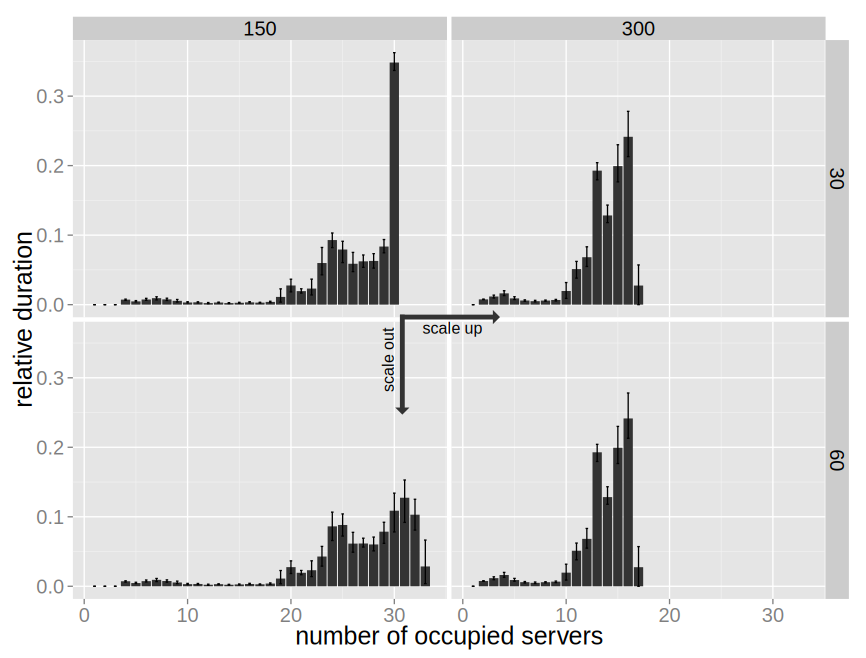
\includegraphics[width=1.0\textwidth]{images/resourceusedistribution-detail-barplot-annotated.pdf}
  \caption{Resource usage from select maximum instances and tunnels combination, displaying the capability to scale.}
 \label{c4:fig:res-usage-barplot}
\end{figure}


\begin{figure}[htb]
  \centering
  \includegraphics[width=1.0\textwidth]{images/startstopduration-blockingprobability-barchart.pdf}
  \caption{Influence of the boot and shutdown time on the blocking probability.}
 \label{c4:fig:blockprob-startstop-barchart}
\end{figure}

\begin{figure}[htb]
  \centering
  \includegraphics[width=1.0\textwidth]{images/feasiblemultiserver-blockprob.pdf}
  \caption{Comparison of the blocking probability of various server configurations.}
 \label{c4:fig:blockprob-multiserver}
\end{figure}

\begin{figure}[htb]
  \centering
  \includegraphics[width=1.0\textwidth]{images/feasiblemultiserver-blockprob.pdf}
  \caption{Comparison of the resource usage of various server configurations.}
 \label{c4:fig:res-usage-multiserver}
\end{figure}

\begin{figure}[htb]
  \centering
  \includegraphics[width=1.0\textwidth]{images/instanceuse-mean.pdf}
  \caption{Mean instance usage of various server configurations.}
 \label{c4:fig:res-instance-usage-mean}
\end{figure}



%%%%%%%%%%%%%%%%%%%%%%%%%%%%%%%%%%%%%%%%%%%%%%%%%%%%%%%%%%%%%%%%%%%%%%%%%%%%%%%
\subsection{Modeling Discussion}




%%%%%%%%%%%%%%%%%%%%%%%%%%%%%%%%%%%%%%%%%%%%%%%%%%%%%%%%%%%%%%%%%%%%%%%%%%%%%%%%
%!TEX root = ../../dissertation.tex
%%%%%%%%%%%%%%%%%%%%%%%%%%%%%%%%%%%%%%%%%%%%%%%%%%%%%%%%%%%%%%%%%%%%%%%%%%%%%%%
\section{Load Model Queuing Simulation} 
\label{c4:simulation}

As discussed, the solvability of a non-stationary Erlang loss system is very limited. To better tackle this, a simulative approach can be taken. Depending on the level of detail, different types of simulations are available.

Here, a queuing simulation is used to ascertain the blocking probability and tunnel serving slot utilization from the model using the fitted distributions from the trace.


%%%%%%%%%%%%%%%%%%%%%%%%%%%%%%%%%%%%%%%%%%%%%%%%%%%%%%%%%%%%%%%%%%%%%%%%%%%%%%%
\subsection{Queuing Simulation Implementation}

The queuing simulation is implemented on the basis of a \gls{DES}. Instead of reproducing continuous time, this simulation is a series of discrete events. Time is advanced only at these events. 

A queuing model can be easily represented in a \gls{DES}.  Each tunnel request arrival is a modeled as a discrete event. When such an event occurs, three processes are executed. The first process draws a random number from a \gls{PRNG} mapped to \gls{IAT} exponential distribution to schedule the next arrival event. Secondly, the serving units are checked for any free units. If one is found, it will now be occupied. Else, this arrival will be marked as rejected and the third action skipped. This third process now determines the length of the tunnel using another \gls{PRNG} adjusted to the serving time distribution to schedule the event in which the tunnel exits the system.

This model was implemented on the basis of version 3.0 of the \textit{SimPy}~\cite{simpy} package, which is a Python \gls{DES} framework that provides the basic event and scheduling infrastructure. On top of this a base \gls{GGSN} class was constructed, managing the arrival of tunnel events and the scheduling of the service ending events. Specific classes for the traditional (i.e. monolithic) and virtualized (called ``multiserver'' in the code) nodes respectively exist. The implementation is also publicly available\footnote{\url{https://github.com/fmetzger/ggsn-simulation/}} as a reference. 


%%%%%%%%%%%%%%%%%%%%%%%%%%%%%%%%%%%%%%%%%%%%%%%%%%%%%%%%%%%%%%%%%%%%%%%%%%%%%%%
\subsection{Description and Design of the Individual Experiments}

To match the measurement data the simulation time is set to be \SI{7}{\day} in all simulation scenarios. The initial \SI{60}{\minute} of each experiment are considered to be the transient phase and are afterwards deducted from the results. Ten replications of each scenario were performed. All depicted error bars show the \SI{5}{\percent} and \SI{95}{\percent} quantiles of all replications.

The first experiment was conducted to investigate the normalized baseline load a monolithic \gls{GGSN} experiences using the presented model. Using this, a maximum to the number of concurrent tunnels and the correlation to the blocking probability and tunnel rejection rate can be established. The effects of scaling up, improving the hardware capabilities of the single node, can thus be investigated.

Based on these results, the virtualization and scaling out effects in the virtualized, \gls{GGSN} model are examined. In order to study the feasibility of this approach the performance indicators of the virtual \gls{GGSN} are compared to the baseline established in the first experiment. To this end, the virtual \gls{GGSN} is simulated in configurations varying the number of instances and supported concurrent tunnels per instance.

In a final experiment the startup and shutdown duration of virtual instances and the life cycle management of these instances are additionally taken into account. Although the boot duration of modern \glspl{os} and \glspl{VM}, especially on current hardware with flash storage, is significantly lower than it has been in the past, there is still a delay. This could cause further blocking if the load balancer does not account for this. But the more generously the balancer starts instances in advance the smaller the virtualization efficiency gain, especially the energy consumption, will be become. For this reason, the number of active instance is a relevant performance metric in the virtual \gls{GGSN} model.

The experiment varies the boot delay and implements a very simple load balancer rule as baseline. The rule keeps at least one empty instance running in reserve at all times and deactivates instances, when two running instances are completely unused. As this is very generous, virtualization blocking should only occur in cases of very small instances or very rapid arrivals. Realistic provisioning rules can improve on this quite easily. But even this simplistic approach already serves to demonstrate potential benefits.


%%%%%%%%%%%%%%%%%%%%%%%%%%%%%%%%%%%%%%%%%%%%%%%%%%%%%%%%%%%%%%%%%%%%%%%%%%%%%%%
\subsubsection{GGSN Load, Capacity, and Scaling}

First, with the help of the \glspl{IAT} and duration of tunnels calculated in the dataset evaluation, the monolithic \gls{GGSN} model is studied. While these traces provided information on the frequency of new tunnels and the duration they remain active, no reliable information on the number of required supported concurrent tunnels for a given arrival rate could be deduced. 
This experiment evaluates arbitrary values for the \gls{GGSN} tunnel capacity and determines the resulting blocking probability such that a suitable value can be found. This is a typical task in a dimensioning process.

\begin{figure}[htb]
  \centering
  \includegraphics[width=1.0\textwidth]{images/R-monolithic-blocking.pdf}
  \caption{Impact of the number of supported parallel tunnels on the blocking probability for the traditional \gls{GGSN} model. For each scenario the mean of all simulated replications as well as \SI{5}{\percent} and \SI{95}{\percent} quantiles as error bars are shown.}
\label{c4:fig:traditional_blocking}
\end{figure}

Figure~\ref{c4:fig:traditional_blocking} studies this impact of the maximum supported number of concurrent tunnels $n$ on the blocking probability $p_B$. $n$ is incrementally increased in steps of \numprint{100} tunnels from \numprint{0} to \numprint{5500}. As expected, the blocking probability decreases with the number of supported tunnels.An almost linear correlation can be observed in the larger part of the graph with a small convergence phase shortly before reaching $p_B=0$. For the normalized inter-arrival no blocking is occurring if a capacity of \numprint{5000} concurrent tunnels is allocated to the \gls{GGSN}. The results are stable across all simulation runs as the error bars display. For the purpose of network dimensioning the results can be easily scaled up from the normalized arrival rates to the actual ones in the network in question.

\begin{table}[htb]
  \caption{Manipulation check for the experimental factors based on one-way \acrshort{ANOVA}.}
  \centering
  \label{c4:tab:manipulation2color}
  \begin{tabu}{X[1.6,l]X[r]X[r]X[r]X[1.1r]X[1.1,r]}
  \toprule
  & $\mathbf{F(2,1275)}$ & $\mathbf{\eta^2_p}$ & $\mathbf{p}$ & \textbf{Cohen's} $\mathbf{f^2}$ & \textbf{Cohen's} $\mathbf{\hat{\omega}^2}$\\ 
  \midrule
  \multicolumn{2}{l}{\textit{blocking probability}} & & & &\\ 
  maxTunnels &  $15601.534$ & $\color{red}0.99$ & $<0.001$ & $\color{red} 26.739$ & $0.964$\\ 
  maxInstances &  $10218.173$ & $\color{red} 0.986$ & $<0.001$ & $\color{red} 1.068$ & $0.516$\\ 
  startstopDuration & $0.868$ & $\color{black} 0.003$ & $0.482$ & $\color{black} 0.000$ & $0.000$\\
  \midrule
  \multicolumn{2}{l}{\textit{mean number of tunnels}}& & & &\\ 
  maxTunnels & $20448.347$ & $\color{red} 0.994$ & $<0.001$ & $\color{red} 27.712$ & $0.965$\\ 
  maxInstances & $13348.251$ & $\color{red} 0.989$ & $<0.001$ & $\color{red} 1.064$ & $0.515$\\ 
  startstopDuration & $2.872$ & $\color{black} 0.009$ & $0.022$ & $\color{black} 0.000$ & $0.000$\\
  \bottomrule
  \end{tabu}
\end{table}

% <---!

In order to analyze the influence of the different model parameters on the resulting metrics, a one-way \gls{ANOVA} is performed, with the results depicted in Table~\ref{c4:tab:manipulation2color}. High values for $\eta_p^2$ and Cohen's $f^2$ \cite{stats} indicate that the main influence for both blocking probability and mean number of tunnels is the maximum number of tunnels $n$ and servers $S_{\max}$, i.e. the total number of possible concurrent tunnels in the system.
Therefore, we study these parameters first.

\todo{Re-check the anova statistical stuff and update with own computations, mention and explain  all the used stats (cohens omega and f, p, F, and eta squared)}

\begin{figure}[htb]
  \centering
  \includegraphics{images/instanceuse-multiserver-real.pdf}
  \caption{Impact of the maximum number of tunnels and number of servers on number of active servers in the virtual \gls{GGSN} model.}
 \label{c4:fig:instance_use_virtual}
\end{figure}

In Figure~\ref{c4:fig:instance_use_virtual} the \gls{CDF} of the number of active servers for four different virtual \gls{GGSN} configurations is displayed. We observe, that increasing the number of supported tunnels per server allows a larger percentage of servers to be shutdown or used for other tasks. This demonstrates the scaling capability of the virtualized model quite well. Note, that both the scenario with \numprint{30} servers and \numprint{150} maximum tunnels per server as well as the scenario with \numprint{60} servers and \numprint{75} maximum tunnels per server share the same maximum amount of tunnels, \numprint{4500}, being right at the center of the interesting range of candidates.


%%%%%%%%%%%%%%%%%%%%%%%%%%%%%%%%%%%%%%%%%%%%%%%%%%%%%%%%%%%%%%%%%%%%%%%%%%%%%%%
\subsubsection{Virtualization Impact and Gain}

\begin{figure}[htb]
  \centering
  \includegraphics{images/blocking-comparison.pdf}
  \caption{Relative increase of blocking probability on the number of servers compared to the traditional \gls{GGSN}; with the $4500$ maximum tunnels per server being on a single server, $150$ on $30$, and $75$ on $60$ servers.}
 \label{c4:fig:blocking-comparison}
\end{figure}

Next, we take a look at the blocking probability of the virtual \gls{GGSN} system in Figure~\ref{c4:fig:blocking-comparison} and compare it to the results from the traditional \gls{GGSN} model. In Figure~\ref{c4:fig:blocking-comparison} we compare the blocking probability of the traditional \gls{GGSN} system dimensioned for $4500$ concurrent tunnels with the virtual \gls{GGSN}.

We observe that, with the start up and shut down time of $5$ minutes in mind, the blocking probability increases by a factor of $1.48$ if the capacity of each server is set to $75$, i.e. $\frac{1}{60}$ of the original server capacity, while $27$ of all $60$ servers can be turned of or used for other purposes at \SI{50}{\percent} of the time. We conclude, that choosing more powerful servers decreases the blocking probability but reduces the potential to disable servers.

So far we have considered a conservative start up and shut down time of servers of \SI{5}{\minute}, which can potentially occur if current generation physical servers are used.
In the next section we study the impact of reduced start up and shut down times with modern servers with fast storage (e.g. \glspl{SSD}) or virtual servers provisioned in the cloud.


%%%%%%%%%%%%%%%%%%%%%%%%%%%%%%%%%%%%%%%%%%%%%%%%%%%%%%%%%%%%%%%%%%%%%%%%%%%%%%%
\subsubsection{Virtual Instance Life Cycle Management Impact}

In this section, we first consider the impact of different boot and shut down times on resource utilization and blocking probabilities. We observe the impact of different start up and shut down times on both resource utilization and blocking probability. Afterwards, the influence of varying server start and stop times on a fixed combination of maximum tunnels and servers in the system is examined.

\begin{figure}[htb]
  \centering
  \includegraphics{images/compare-util-block.pdf}
  \caption{Trade-off between blocking probability and mean resource utilization with regard to maximum number of servers, maximum number of tunnels per server, and start up and shut down time.}
 \label{c4:fig:compare_util_block}
\end{figure}

Figure~\ref{c4:fig:compare_util_block} shows scenarios with $40$ and $100$ number of virtual \gls{GGSN} instances and  $1000$ to $5000$ total concurrent tunnels. For each scenario, we study the impact of selecting different maximum numbers of tunnel per server as well as start up and shut down times on blocking probability and mean resource utilization. The first observation is that by increasing the number of servers, i.e. scaling out, the blocking probability can be decreased, while maintaining a relatively low mean resource utilization. In addition to the previous effects, we notice that a higher start up and shut down time causes a slight increase in blocking probability for servers with low tunnel capacity.

\begin{figure}[htb]
  \centering
  \includegraphics{images/compare-maxinstances-block.pdf}
  \caption{Influence of start up and shut down time on blocking probability with regard to different numbers of servers.}
 \label{c4:fig:compare_maxinstances_block}
\end{figure}

In order to study this behavior in more detail, we focus on a specific scenario in Figure~\ref{c4:fig:compare_maxinstances_block}, where $5000$ total tunnels should be supported by the system. In order to achieve this goal, we consider three types of instances, with the server capacity varying between $50$ and $500$.  In each case we change the start up and shut down time between $1$ and $5$ minutes. It can be easily observed, that lower server capacities combined with higher start up and shut down times increase the blocking probability. This is due to the server start up threshold mechanism, used in the model, not taking the additional capacity gained by activating an additional server into account. If a low capacity server with a long boot time is activated, there is a high probability that the system will quickly expend its capacity again.

Thus, it can be concluded, that if smaller instances are to be used, for example because they are cheaper than large instances, start up and shut down times should be kept minimal, for example by using virtual instances or \glspl{SSD}.



%%%%%%%%%%%%%%%%%%%%%%%%%%%%%%%%%%%%%%%%%%%%%%%%
% additional figures for simulation

\begin{figure}[htb]
  \centering
  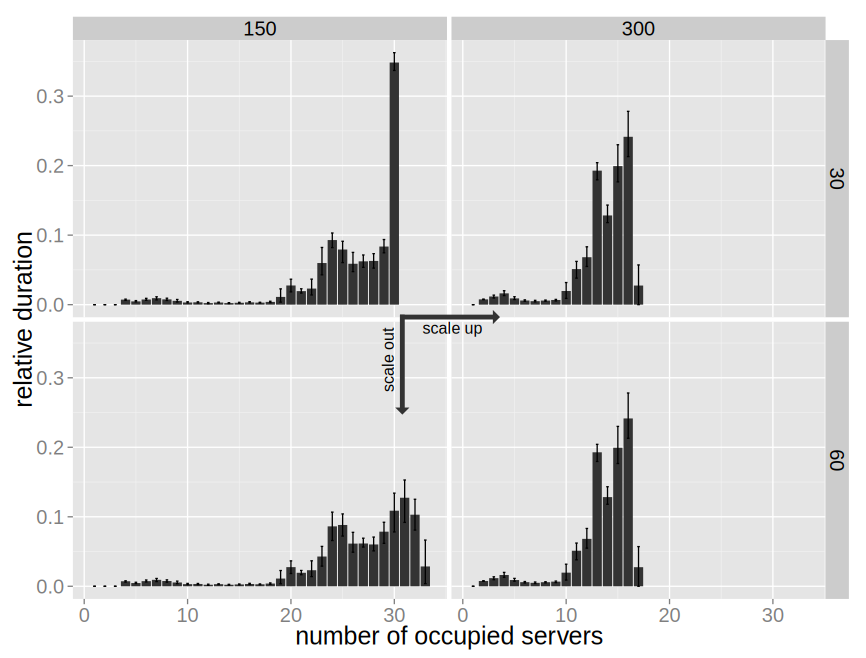
\includegraphics[width=1.0\textwidth]{images/resourceusedistribution-detail-barplot-annotated.pdf}
  \caption{Resource usage from select maximum instances and tunnels combination, displaying the capability to scale.}
 \label{c4:fig:res-usage-barplot}
\end{figure}


\begin{figure}[htb]
  \centering
  \includegraphics[width=1.0\textwidth]{images/startstopduration-blockingprobability-barchart.pdf}
  \caption{Influence of the boot and shutdown time on the blocking probability.}
 \label{c4:fig:blockprob-startstop-barchart}
\end{figure}

\begin{figure}[htb]
  \centering
  \includegraphics[width=1.0\textwidth]{images/feasiblemultiserver-blockprob.pdf}
  \caption{Comparison of the blocking probability of various server configurations.}
 \label{c4:fig:blockprob-multiserver}
\end{figure}

\begin{figure}[htb]
  \centering
  \includegraphics[width=1.0\textwidth]{images/feasiblemultiserver-blockprob.pdf}
  \caption{Comparison of the resource usage of various server configurations.}
 \label{c4:fig:res-usage-multiserver}
\end{figure}

\begin{figure}[htb]
  \centering
  \includegraphics[width=1.0\textwidth]{images/instanceuse-mean.pdf}
  \caption{Mean instance usage of various server configurations.}
 \label{c4:fig:res-instance-usage-mean}
\end{figure}


%The range of \numprint{4000} to \numprint{5000} concurrent tunnels to be of special interest for the remainder of the study.

%%%%%%%%%%%%%%%%%%%%%%%%%%%%%%%%%%%%%%%%%%%%%%%%%%%%%%%%%%%%%%%%%%%%%%%%%%%%%%%%
\section{Core Network Evaluation Summary}
\label{c4:sec:conclusion}


The investigation of a week-long measurement trace recorded in an operational core network revealed some interesting signaling characteristics especially regarding the interdependency between user plane and control plane. Additionally, \gls{gtp} tunnel properties were determined to be a worthwhile measure for control plane load at the \gls{GGSN}, one of the central nodes in a \gls{3G} core network.

The investigation showed that the control plane is easily influenced by several device-based --- as far as they can be distinguished in a core network trace --- and time-of-day related features. The overall diurnal tunnel signaling load closely resembles the progression of the user plane. Most of the control plane's procedures are still triggered, either directly or indirectly, by user devices, of which the offered load is much smaller during night time. The trace evaluation also confirms the dominating influence of smartphones compared to other devices types, even when looking at the control plane.

But this also means that sheer traffic volume is not a good measure to determine load, as the per-device traffic volume of a smartphone is rather low when compared to devices like pure \gls{3G} modems attached to a notebook. In this aspect, the findings also support the stories of signaling storms in mobile networks caused by applications regularly causing small amounts of network traffic. Each application interaction results in disproportionate amounts of signaling load being generated. Even worse, measures taken to improve the radio interface control plane such as Fast Dormancy could possibly have adverse effects to core signaling as they might increase the tunnel churn.

But the load investigation should not stop here. The presented approaches were just the ones that could be conducted with the available data. If one were to have access to a mobile network monitoring system or more detailed data records from such a system, it would open up many more angles in the investigation. For example, recording every individual signaling message with all \glspl{IE} would give hard numbers on the direct signaling overhead, as could measurement probes located inside the network nodes report on the CPU and memory load in order to determine the control plane's processing overhead. A closer investigation of control plane load in relation to mobility behavior should also prove very interesting, as this is one of the central motifs in every mobile network.

Learning from this historical data, queuing theoretic models were created that can describe the control plane load in such networks. These models can be easily used in network dimensioning and planning processes by means of, e.g., stationary analyses. The novel baseline control plane load model presented here is a $M(t)/G(t)/c/0$ non-stationary Erlang loss model. When used in conjunction with parameters derived from the measurement traces it can easily be used for network dimensioning. To improve scaling in the future a further \gls{GGSN} load model with features used in virtualization was also proposed.

Due to general solvability issues of non-stationary Erlang models the model is evaluated and validated using a queuing simulation in terms of their blocking and tunnel state probability as well as the general resource utilization. The virtual model provided the added benefit of being more flexible in its scaling properties and energy efficiency. This might even lead to new \gls{GGSN}-as-a-Service business models, removing the need to provide and operate large amounts of infrastructure for rare cases of peak load. 

All of these properties serve to show the complexity of current mobile network systems even without running media streaming on top of it. Streaming in itself, while not being a real-time duplex communication protocol, is relatively sensitive to timings and influences from lower network layers, which can make streaming over mobile networks rather problematic. The next chapters investigate these issues and methods to evaluate them more closely.

%In the future we would like to deepen our modeling efforts to provide more dimensioning options for a core network. Also, we want to further investigate the correlation of user traffic and signaling and take a look at the implications specific traffic types bring for the core network. 

%All these investigations and modeling efforts combined could lead to a more informed approach of network planning: Being more aware of the control plane provides the necessary tools to identify probable causes for control plane activity. 

%We would also like to expand our evaluations, as there are several angles not investigated so far that could prove worthwhile. This includes an examination of the exact number and size of signaling messages flowing through the core, a more detailed picture of the processing load these messages induce at the \gls{GGSN}, and an evolved model. Furthermore, a differential analysis of our data compared to a newer dataset (potentially including \gls{LTE} access) could really prove worthwhile.

%We also look forward to searching for multiple active tunnels per device. As discussed previously, the \textit{Secondary PDP Context Activation Procedure} enables devices to establish up to ten additional tunnels attributed with a different, higher QoS level, if the network supports this. The additional load of managing and holding multiple tunnels plus the displacement of other, ``lower-quality'' traffic could prove to be an interesting investigation. Initial observations indicate that this feature is rarely used today by very few types of devices, but it will be of increased interest in the face of ongoing LTE/EPS deployments, whose specifications expand upon this secondary tunnel concept.